\documentclass[1p]{elsarticle_modified}
%\bibliographystyle{elsarticle-num}

%\usepackage[colorlinks]{hyperref}
%\usepackage{abbrmath_seonhwa} %\Abb, \Ascr, \Acal ,\Abf, \Afrak
\usepackage{amsfonts}
\usepackage{amssymb}
\usepackage{amsmath}
\usepackage{amsthm}
\usepackage{scalefnt}
\usepackage{amsbsy}
\usepackage{kotex}
\usepackage{caption}
\usepackage{subfig}
\usepackage{color}
\usepackage{graphicx}
\usepackage{xcolor} %% white, black, red, green, blue, cyan, magenta, yellow
\usepackage{float}
\usepackage{setspace}
\usepackage{hyperref}

\usepackage{tikz}
\usetikzlibrary{arrows}

\usepackage{multirow}
\usepackage{array} % fixed length table
\usepackage{hhline}

%%%%%%%%%%%%%%%%%%%%%
\makeatletter
\renewcommand*\env@matrix[1][\arraystretch]{%
	\edef\arraystretch{#1}%
	\hskip -\arraycolsep
	\let\@ifnextchar\new@ifnextchar
	\array{*\c@MaxMatrixCols c}}
\makeatother %https://tex.stackexchange.com/questions/14071/how-can-i-increase-the-line-spacing-in-a-matrix
%%%%%%%%%%%%%%%

\usepackage[normalem]{ulem}

\newcommand{\msout}[1]{\ifmmode\text{\sout{\ensuremath{#1}}}\else\sout{#1}\fi}
%SOURCE: \msout is \stkout macro in https://tex.stackexchange.com/questions/20609/strikeout-in-math-mode

\newcommand{\cancel}[1]{
	\ifmmode
	{\color{red}\msout{#1}}
	\else
	{\color{red}\sout{#1}}
	\fi
}

\newcommand{\add}[1]{
	{\color{blue}\uwave{#1}}
}

\newcommand{\replace}[2]{
	\ifmmode
	{\color{red}\msout{#1}}{\color{blue}\uwave{#2}}
	\else
	{\color{red}\sout{#1}}{\color{blue}\uwave{#2}}
	\fi
}

\newcommand{\Sol}{\mathcal{S}} %segment
\newcommand{\D}{D} %diagram
\newcommand{\A}{\mathcal{A}} %arc


%%%%%%%%%%%%%%%%%%%%%%%%%%%%%5 test

\def\sl{\operatorname{\textup{SL}}(2,\Cbb)}
\def\psl{\operatorname{\textup{PSL}}(2,\Cbb)}
\def\quan{\mkern 1mu \triangleright \mkern 1mu}

\theoremstyle{definition}
\newtheorem{thm}{Theorem}[section]
\newtheorem{prop}[thm]{Proposition}
\newtheorem{lem}[thm]{Lemma}
\newtheorem{ques}[thm]{Question}
\newtheorem{cor}[thm]{Corollary}
\newtheorem{defn}[thm]{Definition}
\newtheorem{exam}[thm]{Example}
\newtheorem{rmk}[thm]{Remark}
\newtheorem{alg}[thm]{Algorithm}

\newcommand{\I}{\sqrt{-1}}
\begin{document}

%\begin{frontmatter}
%
%\title{Boundary parabolic representations of knots up to 8 crossings}
%
%%% Group authors per affiliation:
%\author{Yunhi Cho} 
%\address{Department of Mathematics, University of Seoul, Seoul, Korea}
%\ead{yhcho@uos.ac.kr}
%
%
%\author{Seonhwa Kim} %\fnref{s_kim}}
%\address{Center for Geometry and Physics, Institute for Basic Science, Pohang, 37673, Korea}
%\ead{ryeona17@ibs.re.kr}
%
%\author{Hyuk Kim}
%\address{Department of Mathematical Sciences, Seoul National University, Seoul 08826, Korea}
%\ead{hyukkim@snu.ac.kr}
%
%\author{Seokbeom Yoon}
%\address{Department of Mathematical Sciences, Seoul National University, Seoul, 08826,  Korea}
%\ead{sbyoon15@snu.ac.kr}
%
%\begin{abstract}
%We find all boundary parabolic representation of knots up to 8 crossings.
%
%\end{abstract}
%\begin{keyword}
%    \MSC[2010] 57M25 
%\end{keyword}
%
%\end{frontmatter}

%\linenumbers
%\tableofcontents
%
\newcommand\colored[1]{\textcolor{white}{\rule[-0.35ex]{0.8em}{1.4ex}}\kern-0.8em\color{red} #1}%
%\newcommand\colored[1]{\textcolor{white}{ #1}\kern-2.17ex	\textcolor{white}{ #1}\kern-1.81ex	\textcolor{white}{ #1}\kern-2.15ex\color{red}#1	}

{\Large $\underline{12a_{1100}~(K12a_{1100})}$}

\setlength{\tabcolsep}{10pt}
\renewcommand{\arraystretch}{1.6}
\vspace{1cm}\begin{tabular}{m{100pt}>{\centering\arraybackslash}m{274pt}}
\multirow{5}{120pt}{
	\centering
	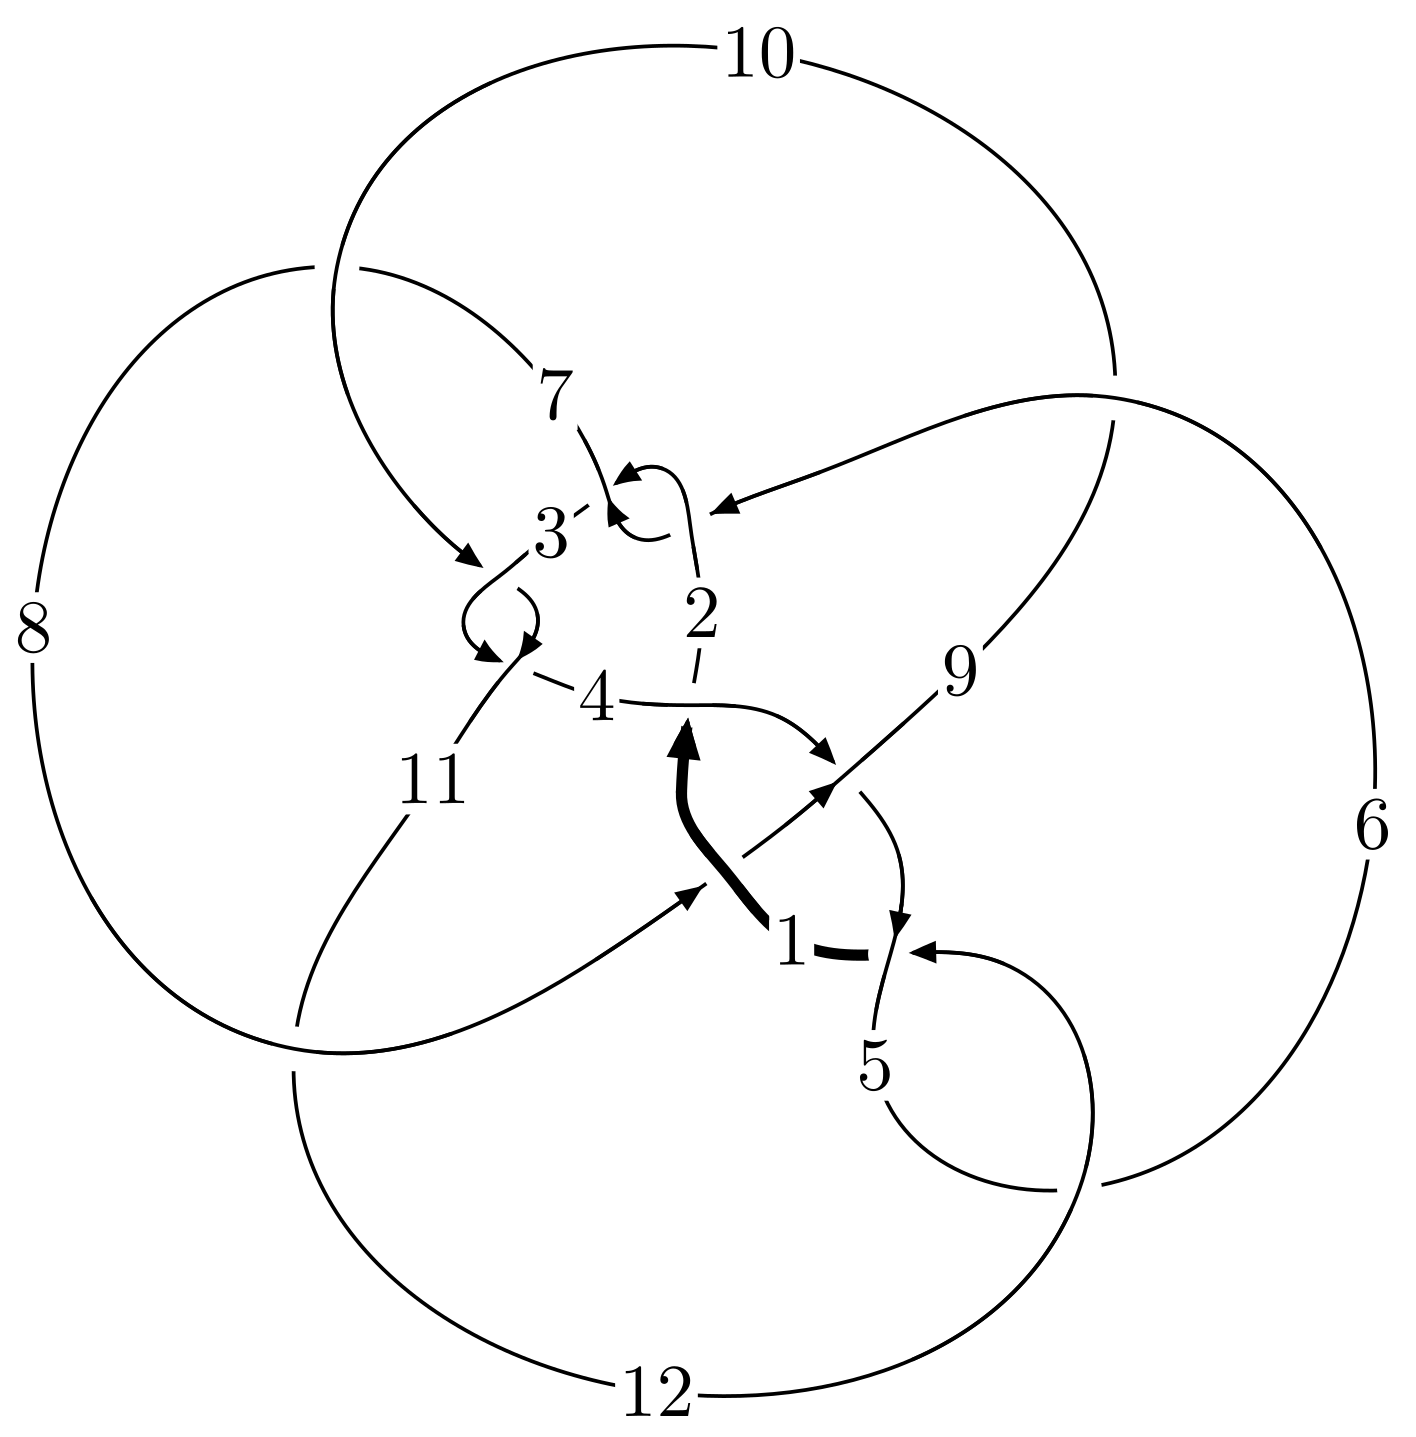
\includegraphics[width=112pt]{../../../GIT/diagram.site/Diagrams/png/1901_12a_1100.png}\\
\ \ \ A knot diagram\footnotemark}&
\allowdisplaybreaks
\textbf{Linearized knot diagam} \\
\cline{2-2}
 &
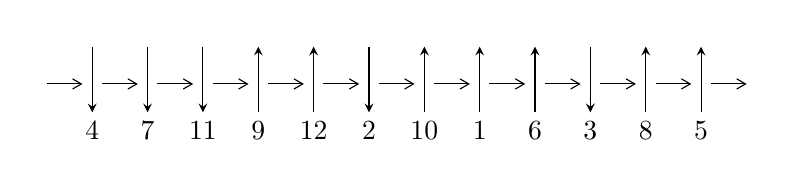
\begin{tikzpicture}[x=20pt, y=17pt]
	% nodes
	\node (C0) at (0, 0) {};
	\node (C1) at (1, 0) {};
	\node (C1U) at (1, +1) {};
	\node (C1D) at (1, -1) {4};

	\node (C2) at (2, 0) {};
	\node (C2U) at (2, +1) {};
	\node (C2D) at (2, -1) {7};

	\node (C3) at (3, 0) {};
	\node (C3U) at (3, +1) {};
	\node (C3D) at (3, -1) {11};

	\node (C4) at (4, 0) {};
	\node (C4U) at (4, +1) {};
	\node (C4D) at (4, -1) {9};

	\node (C5) at (5, 0) {};
	\node (C5U) at (5, +1) {};
	\node (C5D) at (5, -1) {12};

	\node (C6) at (6, 0) {};
	\node (C6U) at (6, +1) {};
	\node (C6D) at (6, -1) {2};

	\node (C7) at (7, 0) {};
	\node (C7U) at (7, +1) {};
	\node (C7D) at (7, -1) {10};

	\node (C8) at (8, 0) {};
	\node (C8U) at (8, +1) {};
	\node (C8D) at (8, -1) {1};

	\node (C9) at (9, 0) {};
	\node (C9U) at (9, +1) {};
	\node (C9D) at (9, -1) {6};

	\node (C10) at (10, 0) {};
	\node (C10U) at (10, +1) {};
	\node (C10D) at (10, -1) {3};

	\node (C11) at (11, 0) {};
	\node (C11U) at (11, +1) {};
	\node (C11D) at (11, -1) {8};

	\node (C12) at (12, 0) {};
	\node (C12U) at (12, +1) {};
	\node (C12D) at (12, -1) {5};
	\node (C13) at (13, 0) {};

	% arrows
	\draw[->,>={angle 60}]
	(C0) edge (C1) (C1) edge (C2) (C2) edge (C3) (C3) edge (C4) (C4) edge (C5) (C5) edge (C6) (C6) edge (C7) (C7) edge (C8) (C8) edge (C9) (C9) edge (C10) (C10) edge (C11) (C11) edge (C12) (C12) edge (C13) ;	\draw[->,>=stealth]
	(C1U) edge (C1D) (C2U) edge (C2D) (C3U) edge (C3D) (C4D) edge (C4U) (C5D) edge (C5U) (C6U) edge (C6D) (C7D) edge (C7U) (C8D) edge (C8U) (C9D) edge (C9U) (C10U) edge (C10D) (C11D) edge (C11U) (C12D) edge (C12U) ;
	\end{tikzpicture} \\
\hhline{~~} \\& 
\textbf{Solving Sequence} \\ \cline{2-2} 
 &
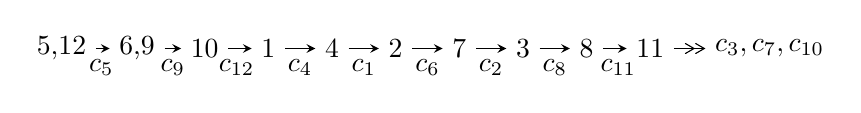
\begin{tikzpicture}[x=23pt, y=7pt]
	% node
	\node (A0) at (-1/8, 0) {5,12};
	\node (A1) at (17/16, 0) {6,9};
	\node (A2) at (17/8, 0) {10};
	\node (A3) at (25/8, 0) {1};
	\node (A4) at (33/8, 0) {4};
	\node (A5) at (41/8, 0) {2};
	\node (A6) at (49/8, 0) {7};
	\node (A7) at (57/8, 0) {3};
	\node (A8) at (65/8, 0) {8};
	\node (A9) at (73/8, 0) {11};
	\node (C1) at (1/2, -1) {$c_{5}$};
	\node (C2) at (13/8, -1) {$c_{9}$};
	\node (C3) at (21/8, -1) {$c_{12}$};
	\node (C4) at (29/8, -1) {$c_{4}$};
	\node (C5) at (37/8, -1) {$c_{1}$};
	\node (C6) at (45/8, -1) {$c_{6}$};
	\node (C7) at (53/8, -1) {$c_{2}$};
	\node (C8) at (61/8, -1) {$c_{8}$};
	\node (C9) at (69/8, -1) {$c_{11}$};
	\node (A10) at (11, 0) {$c_{3},c_{7},c_{10}$};

	% edge
	\draw[->,>=stealth]	
	(A0) edge (A1) (A1) edge (A2) (A2) edge (A3) (A3) edge (A4) (A4) edge (A5) (A5) edge (A6) (A6) edge (A7) (A7) edge (A8) (A8) edge (A9) ;
	\draw[->>,>={angle 60}]	
	(A9) edge (A10);
\end{tikzpicture} \\ 

\end{tabular} \\

\footnotetext{
The image of knot diagram is generated by the software ``\textbf{Draw programme}" developed by Andrew Bartholomew(\url{http://www.layer8.co.uk/maths/draw/index.htm\#Running-draw}), where we modified some parts for our purpose(\url{https://github.com/CATsTAILs/LinksPainter}).
}\phantom \\ \newline 
\centering \textbf{Ideals for irreducible components\footnotemark of $X_{\text{par}}$} 
 
\begin{align*}
I^u_{1}&=\langle 
5.72959\times10^{14} u^{38}+1.09041\times10^{16} u^{37}+\cdots+2.39027\times10^{15} b+2.06660\times10^{16},\\
\phantom{I^u_{1}}&\phantom{= \langle  }-1.43733\times10^{15} u^{38}-1.83777\times10^{16} u^{37}+\cdots+4.78054\times10^{15} a-3.39110\times10^{16},\\
\phantom{I^u_{1}}&\phantom{= \langle  }u^{39}+16 u^{38}+\cdots+384 u+16\rangle \\
I^u_{2}&=\langle 
2.68281\times10^{59} a u^{64}+6.81399\times10^{65} u^{64}+\cdots-1.07313\times10^{60} a+1.71010\times10^{66},\\
\phantom{I^u_{2}}&\phantom{= \langle  }-9.81930\times10^{61} a u^{64}-2.55544\times10^{62} u^{64}+\cdots+6.76295\times10^{62} a-1.80547\times10^{63},\\
\phantom{I^u_{2}}&\phantom{= \langle  }u^{65}-6 u^{64}+\cdots-36 u+4\rangle \\
I^u_{3}&=\langle 
4 u^{19}+19 u^{18}+\cdots+3 b-84,\;40 u^{19}+265 u^{18}+\cdots+9 a-252,\;u^{20}+7 u^{19}+\cdots+42 u+9\rangle \\
I^u_{4}&=\langle 
- u^6 a+3 u^5 a+3 u^6-4 u^4 a-17 u^5+7 u^3 a+37 u^4-2 u^2 a-50 u^3+8 a u+49 u^2+7 b-3 a-27 u+20,\\
\phantom{I^u_{4}}&\phantom{= \langle  }105 u^6 a+64 u^6+\cdots-84 a-80,\;u^7-4 u^6+7 u^5-11 u^4+9 u^3-10 u^2+4 u-3\rangle \\
\\
I^v_{1}&=\langle 
a,\;b+1,\;v^2- v+1\rangle \\
I^v_{2}&=\langle 
a,\;b+v-1,\;v^2- v+1\rangle \\
I^v_{3}&=\langle 
a,\;b+1,\;v+1\rangle \\
\end{align*}
\raggedright * 7 irreducible components of $\dim_{\mathbb{C}}=0$, with total 208 representations.\\
\footnotetext{All coefficients of polynomials are rational numbers. But the coefficients are sometimes approximated in decimal forms when there is not enough margin.}
\newpage
\renewcommand{\arraystretch}{1}
\centering \section*{I. $I^u_{1}= \langle 5.73\times10^{14} u^{38}+1.09\times10^{16} u^{37}+\cdots+2.39\times10^{15} b+2.07\times10^{16},\;-1.44\times10^{15} u^{38}-1.84\times10^{16} u^{37}+\cdots+4.78\times10^{15} a-3.39\times10^{16},\;u^{39}+16 u^{38}+\cdots+384 u+16 \rangle$}
\flushleft \textbf{(i) Arc colorings}\\
\begin{tabular}{m{7pt} m{180pt} m{7pt} m{180pt} }
\flushright $a_{5}=$&$\begin{pmatrix}1\\0\end{pmatrix}$ \\
\flushright $a_{12}=$&$\begin{pmatrix}0\\u\end{pmatrix}$ \\
\flushright $a_{6}=$&$\begin{pmatrix}1\\- u^2\end{pmatrix}$ \\
\flushright $a_{9}=$&$\begin{pmatrix}0.300662 u^{38}+3.84428 u^{37}+\cdots-77.7458 u+7.09355\\-0.239704 u^{38}-4.56188 u^{37}+\cdots-191.761 u-8.64586\end{pmatrix}$ \\
\flushright $a_{10}=$&$\begin{pmatrix}0.428147 u^{38}+6.52414 u^{37}+\cdots+96.7473 u+13.9087\\0.905515 u^{38}+13.2597 u^{37}+\cdots+56.0756 u+1.59569\end{pmatrix}$ \\
\flushright $a_{1}=$&$\begin{pmatrix}u\\u\end{pmatrix}$ \\
\flushright $a_{4}=$&$\begin{pmatrix}0.239436 u^{38}+4.06041 u^{37}+\cdots+114.171 u-2.79844\\0.0678388 u^{38}+1.24701 u^{37}+\cdots-66.9463 u-2.74556\end{pmatrix}$ \\
\flushright $a_{2}=$&$\begin{pmatrix}-0.730365 u^{38}-9.31593 u^{37}+\cdots+536.715 u+28.7964\\1.69641 u^{38}+27.9777 u^{37}+\cdots+895.140 u+37.7430\end{pmatrix}$ \\
\flushright $a_{7}=$&$\begin{pmatrix}-0.368631 u^{38}-6.47910 u^{37}+\cdots-578.385 u-26.6962\\-1.09599 u^{38}-18.3459 u^{37}+\cdots-583.090 u-24.3794\end{pmatrix}$ \\
\flushright $a_{3}=$&$\begin{pmatrix}-0.536809 u^{38}-8.88416 u^{37}+\cdots-128.853 u-1.15988\\-1.23413 u^{38}-19.3337 u^{37}+\cdots-191.781 u-7.92257\end{pmatrix}$ \\
\flushright $a_{8}=$&$\begin{pmatrix}-0.425949 u^{38}-6.68769 u^{37}+\cdots+5.65478 u+10.9288\\-0.966315 u^{38}-15.0939 u^{37}+\cdots-108.361 u-4.81059\end{pmatrix}$ \\
\flushright $a_{11}=$&$\begin{pmatrix}-0.152023 u^{38}-2.64110 u^{37}+\cdots-41.2325 u+6.25229\\0.249003 u^{38}+3.45982 u^{37}+\cdots+45.1427 u+1.36843\end{pmatrix}$\\&\end{tabular}
\flushleft \textbf{(ii) Obstruction class $= -1$}\\~\\
\flushleft \textbf{(iii) Cusp Shapes $= \frac{55786339166132}{27162180570893} u^{38}+\frac{844053926444108}{27162180570893} u^{37}+\cdots+\frac{4041570281227700}{27162180570893} u+\frac{344262331286382}{27162180570893}$}\\~\\
\newpage\renewcommand{\arraystretch}{1}
\flushleft \textbf{(iv) u-Polynomials at the component}\newline \\
\begin{tabular}{m{50pt}|m{274pt}}
Crossings & \hspace{64pt}u-Polynomials at each crossing \\
\hline $$\begin{aligned}c_{1}\end{aligned}$$&$\begin{aligned}
&u^{39}-30 u^{38}+\cdots-270336 u+16384
\end{aligned}$\\
\hline $$\begin{aligned}c_{2},c_{3},c_{6}\\c_{10}\end{aligned}$$&$\begin{aligned}
&u^{39}-17 u^{37}+\cdots+3 u-1
\end{aligned}$\\
\hline $$\begin{aligned}c_{4},c_{8}\end{aligned}$$&$\begin{aligned}
&u^{39}+7 u^{37}+\cdots-10 u-1
\end{aligned}$\\
\hline $$\begin{aligned}c_{5},c_{12}\end{aligned}$$&$\begin{aligned}
&u^{39}-16 u^{38}+\cdots+384 u-16
\end{aligned}$\\
\hline $$\begin{aligned}c_{7}\end{aligned}$$&$\begin{aligned}
&u^{39}+28 u^{38}+\cdots-39904 u-2512
\end{aligned}$\\
\hline $$\begin{aligned}c_{9},c_{11}\end{aligned}$$&$\begin{aligned}
&u^{39}+2 u^{38}+\cdots-20 u-7
\end{aligned}$\\
\hline
\end{tabular}\\~\\
\newpage\renewcommand{\arraystretch}{1}
\flushleft \textbf{(v) Riley Polynomials at the component}\newline \\
\begin{tabular}{m{50pt}|m{274pt}}
Crossings & \hspace{64pt}Riley Polynomials at each crossing \\
\hline $$\begin{aligned}c_{1}\end{aligned}$$&$\begin{aligned}
&y^{39}+48 y^{37}+\cdots+1677721600 y-268435456
\end{aligned}$\\
\hline $$\begin{aligned}c_{2},c_{3},c_{6}\\c_{10}\end{aligned}$$&$\begin{aligned}
&y^{39}-34 y^{38}+\cdots-13 y-1
\end{aligned}$\\
\hline $$\begin{aligned}c_{4},c_{8}\end{aligned}$$&$\begin{aligned}
&y^{39}+14 y^{38}+\cdots+28 y-1
\end{aligned}$\\
\hline $$\begin{aligned}c_{5},c_{12}\end{aligned}$$&$\begin{aligned}
&y^{39}+24 y^{38}+\cdots+30592 y-256
\end{aligned}$\\
\hline $$\begin{aligned}c_{7}\end{aligned}$$&$\begin{aligned}
&y^{39}-10 y^{38}+\cdots-133816704 y-6310144
\end{aligned}$\\
\hline $$\begin{aligned}c_{9},c_{11}\end{aligned}$$&$\begin{aligned}
&y^{39}-10 y^{38}+\cdots+120 y-49
\end{aligned}$\\
\hline
\end{tabular}\\~\\
\newpage\flushleft \textbf{(vi) Complex Volumes and Cusp Shapes}
$$\begin{array}{c|c|c}  
\text{Solutions to }I^u_{1}& \I (\text{vol} + \sqrt{-1}CS) & \text{Cusp shape}\\
 \hline 
\begin{aligned}
u &= \phantom{-}0.036584 + 1.055630 I \\
a &= -0.33336 - 2.00119 I \\
b &= \phantom{-}0.78963 - 1.21425 I\end{aligned}
 & -8.44685 - 3.59036 I & \phantom{-0.000000 } 0 \\ \hline\begin{aligned}
u &= \phantom{-}0.036584 - 1.055630 I \\
a &= -0.33336 + 2.00119 I \\
b &= \phantom{-}0.78963 + 1.21425 I\end{aligned}
 & -8.44685 + 3.59036 I & \phantom{-0.000000 } 0 \\ \hline\begin{aligned}
u &= -0.878996 + 0.590569 I \\
a &= -0.494056 - 0.310732 I \\
b &= \phantom{-}0.175406 - 1.010140 I\end{aligned}
 & -7.20717 + 4.28473 I & \phantom{-0.000000 } 0 \\ \hline\begin{aligned}
u &= -0.878996 - 0.590569 I \\
a &= -0.494056 + 0.310732 I \\
b &= \phantom{-}0.175406 + 1.010140 I\end{aligned}
 & -7.20717 - 4.28473 I & \phantom{-0.000000 } 0 \\ \hline\begin{aligned}
u &= -0.956553 + 0.471077 I \\
a &= \phantom{-}0.535712 - 0.170609 I \\
b &= \phantom{-}0.790827 + 0.990127 I\end{aligned}
 & -1.05743 + 4.09464 I & \phantom{-0.000000 } 0 \\ \hline\begin{aligned}
u &= -0.956553 - 0.471077 I \\
a &= \phantom{-}0.535712 + 0.170609 I \\
b &= \phantom{-}0.790827 - 0.990127 I\end{aligned}
 & -1.05743 - 4.09464 I & \phantom{-0.000000 } 0 \\ \hline\begin{aligned}
u &= \phantom{-}0.924956 + 0.600813 I \\
a &= \phantom{-}0.371281 + 0.003907 I \\
b &= \phantom{-}0.194948 + 0.056914 I\end{aligned}
 & -1.90733 - 0.89775 I & \phantom{-0.000000 } 0 \\ \hline\begin{aligned}
u &= \phantom{-}0.924956 - 0.600813 I \\
a &= \phantom{-}0.371281 - 0.003907 I \\
b &= \phantom{-}0.194948 - 0.056914 I\end{aligned}
 & -1.90733 + 0.89775 I & \phantom{-0.000000 } 0 \\ \hline\begin{aligned}
u &= \phantom{-}0.165288 + 0.859735 I \\
a &= \phantom{-}0.19991 + 1.68117 I \\
b &= -0.600415 + 0.828931 I\end{aligned}
 & \phantom{-}0.894106 + 0.967260 I & -3.54690 + 1.12714 I \\ \hline\begin{aligned}
u &= \phantom{-}0.165288 - 0.859735 I \\
a &= \phantom{-}0.19991 - 1.68117 I \\
b &= -0.600415 - 0.828931 I\end{aligned}
 & \phantom{-}0.894106 - 0.967260 I & -3.54690 - 1.12714 I\\
 \hline 
 \end{array}$$\newpage$$\begin{array}{c|c|c}  
\text{Solutions to }I^u_{1}& \I (\text{vol} + \sqrt{-1}CS) & \text{Cusp shape}\\
 \hline 
\begin{aligned}
u &= -1.147020 + 0.124747 I \\
a &= \phantom{-}0.171216 + 0.003090 I \\
b &= \phantom{-}0.837941 + 0.589840 I\end{aligned}
 & \phantom{-}5.13665 + 3.68306 I & \phantom{-0.000000 } 0 \\ \hline\begin{aligned}
u &= -1.147020 - 0.124747 I \\
a &= \phantom{-}0.171216 - 0.003090 I \\
b &= \phantom{-}0.837941 - 0.589840 I\end{aligned}
 & \phantom{-}5.13665 - 3.68306 I & \phantom{-0.000000 } 0 \\ \hline\begin{aligned}
u &= -1.198810 + 0.091688 I \\
a &= -0.203582 - 0.083707 I \\
b &= -0.887863 - 0.820311 I\end{aligned}
 & -2.5570 + 14.4897 I & \phantom{-0.000000 } 0 \\ \hline\begin{aligned}
u &= -1.198810 - 0.091688 I \\
a &= -0.203582 + 0.083707 I \\
b &= -0.887863 + 0.820311 I\end{aligned}
 & -2.5570 - 14.4897 I & \phantom{-0.000000 } 0 \\ \hline\begin{aligned}
u &= -0.086623 + 1.203880 I \\
a &= \phantom{-}0.166421 - 0.717215 I \\
b &= \phantom{-}0.477964 - 0.342610 I\end{aligned}
 & -1.53805 - 1.55148 I & \phantom{-0.000000 } 0 \\ \hline\begin{aligned}
u &= -0.086623 - 1.203880 I \\
a &= \phantom{-}0.166421 + 0.717215 I \\
b &= \phantom{-}0.477964 + 0.342610 I\end{aligned}
 & -1.53805 + 1.55148 I & \phantom{-0.000000 } 0 \\ \hline\begin{aligned}
u &= -0.436516 + 1.163100 I \\
a &= -0.01640 - 1.55798 I \\
b &= \phantom{-}1.07400 - 1.04381 I\end{aligned}
 & -1.26442 - 4.12128 I & \phantom{-0.000000 } 0 \\ \hline\begin{aligned}
u &= -0.436516 - 1.163100 I \\
a &= -0.01640 + 1.55798 I \\
b &= \phantom{-}1.07400 + 1.04381 I\end{aligned}
 & -1.26442 + 4.12128 I & \phantom{-0.000000 } 0 \\ \hline\begin{aligned}
u &= \phantom{-}0.086287 + 1.258930 I \\
a &= -0.440278 - 0.963873 I \\
b &= \phantom{-}0.171571 - 0.785654 I\end{aligned}
 & -7.91630 + 2.00919 I & \phantom{-0.000000 } 0 \\ \hline\begin{aligned}
u &= \phantom{-}0.086287 - 1.258930 I \\
a &= -0.440278 + 0.963873 I \\
b &= \phantom{-}0.171571 + 0.785654 I\end{aligned}
 & -7.91630 - 2.00919 I & \phantom{-0.000000 } 0\\
 \hline 
 \end{array}$$\newpage$$\begin{array}{c|c|c}  
\text{Solutions to }I^u_{1}& \I (\text{vol} + \sqrt{-1}CS) & \text{Cusp shape}\\
 \hline 
\begin{aligned}
u &= -0.270947 + 1.287730 I \\
a &= \phantom{-}0.34276 + 1.52890 I \\
b &= -0.670447 + 1.221440 I\end{aligned}
 & -12.67430 + 1.13506 I & \phantom{-0.000000 } 0 \\ \hline\begin{aligned}
u &= -0.270947 - 1.287730 I \\
a &= \phantom{-}0.34276 - 1.52890 I \\
b &= -0.670447 - 1.221440 I\end{aligned}
 & -12.67430 - 1.13506 I & \phantom{-0.000000 } 0 \\ \hline\begin{aligned}
u &= -0.640026 + 1.167660 I \\
a &= \phantom{-}0.30621 + 1.53504 I \\
b &= -0.96815 + 1.40442 I\end{aligned}
 & -3.29095 - 9.95463 I & \phantom{-0.000000 } 0 \\ \hline\begin{aligned}
u &= -0.640026 - 1.167660 I \\
a &= \phantom{-}0.30621 - 1.53504 I \\
b &= -0.96815 - 1.40442 I\end{aligned}
 & -3.29095 + 9.95463 I & \phantom{-0.000000 } 0 \\ \hline\begin{aligned}
u &= -0.107147 + 0.577529 I \\
a &= -1.68285 - 0.68447 I \\
b &= -0.004425 - 1.003520 I\end{aligned}
 & -7.10874 + 3.72846 I & -6.61899 - 2.67591 I \\ \hline\begin{aligned}
u &= -0.107147 - 0.577529 I \\
a &= -1.68285 + 0.68447 I \\
b &= -0.004425 + 1.003520 I\end{aligned}
 & -7.10874 - 3.72846 I & -6.61899 + 2.67591 I \\ \hline\begin{aligned}
u &= -0.505641 + 0.268154 I \\
a &= \phantom{-}0.229112 + 0.984301 I \\
b &= -0.963460 - 0.359880 I\end{aligned}
 & \phantom{-}1.45784 + 0.14435 I & \phantom{-}8.80782 + 0.96026 I \\ \hline\begin{aligned}
u &= -0.505641 - 0.268154 I \\
a &= \phantom{-}0.229112 - 0.984301 I \\
b &= -0.963460 + 0.359880 I\end{aligned}
 & \phantom{-}1.45784 - 0.14435 I & \phantom{-}8.80782 - 0.96026 I \\ \hline\begin{aligned}
u &= -0.72717 + 1.23001 I \\
a &= \phantom{-}0.146791 + 0.665989 I \\
b &= -0.394498 + 0.665266 I\end{aligned}
 & \phantom{-}0.51433 - 3.59139 I & \phantom{-0.000000 } 0 \\ \hline\begin{aligned}
u &= -0.72717 - 1.23001 I \\
a &= \phantom{-}0.146791 - 0.665989 I \\
b &= -0.394498 - 0.665266 I\end{aligned}
 & \phantom{-}0.51433 + 3.59139 I & \phantom{-0.000000 } 0\\
 \hline 
 \end{array}$$\newpage$$\begin{array}{c|c|c}  
\text{Solutions to }I^u_{1}& \I (\text{vol} + \sqrt{-1}CS) & \text{Cusp shape}\\
 \hline 
\begin{aligned}
u &= -0.58754 + 1.31220 I \\
a &= -0.03772 + 1.45994 I \\
b &= -1.04205 + 1.11551 I\end{aligned}
 & \phantom{-}1.41624 - 9.73414 I & \phantom{-0.000000 } 0 \\ \hline\begin{aligned}
u &= -0.58754 - 1.31220 I \\
a &= -0.03772 - 1.45994 I \\
b &= -1.04205 - 1.11551 I\end{aligned}
 & \phantom{-}1.41624 + 9.73414 I & \phantom{-0.000000 } 0 \\ \hline\begin{aligned}
u &= -0.72423 + 1.24628 I \\
a &= -0.564329 - 0.961952 I \\
b &= \phantom{-}0.267022 - 1.230810 I\end{aligned}
 & -9.2783 - 10.7010 I & \phantom{-0.000000 } 0 \\ \hline\begin{aligned}
u &= -0.72423 - 1.24628 I \\
a &= -0.564329 + 0.961952 I \\
b &= \phantom{-}0.267022 + 1.230810 I\end{aligned}
 & -9.2783 + 10.7010 I & \phantom{-0.000000 } 0 \\ \hline\begin{aligned}
u &= -0.59784 + 1.35155 I \\
a &= -0.00220 - 1.60026 I \\
b &= \phantom{-}1.08597 - 1.27810 I\end{aligned}
 & -6.5200 - 20.7521 I & \phantom{-0.000000 } 0 \\ \hline\begin{aligned}
u &= -0.59784 - 1.35155 I \\
a &= -0.00220 + 1.60026 I \\
b &= \phantom{-}1.08597 + 1.27810 I\end{aligned}
 & -6.5200 + 20.7521 I & \phantom{-0.000000 } 0 \\ \hline\begin{aligned}
u &= -0.30394 + 1.70133 I \\
a &= \phantom{-}0.362788 + 0.429884 I \\
b &= \phantom{-}0.071610 + 0.523994 I\end{aligned}
 & -8.37466 + 8.10029 I & \phantom{-0.000000 } 0 \\ \hline\begin{aligned}
u &= -0.30394 - 1.70133 I \\
a &= \phantom{-}0.362788 - 0.429884 I \\
b &= \phantom{-}0.071610 - 0.523994 I\end{aligned}
 & -8.37466 - 8.10029 I & \phantom{-0.000000 } 0 \\ \hline\begin{aligned}
u &= -0.0882066\phantom{ +0.000000I} \\
a &= \phantom{-}8.38515\phantom{ +0.000000I} \\
b &= -0.811176\phantom{ +0.000000I}\end{aligned}
 & \phantom{-}1.27021\phantom{ +0.000000I} & \phantom{-}8.62500\phantom{ +0.000000I}\\
 \hline 
 \end{array}$$\newpage\newpage\renewcommand{\arraystretch}{1}
\centering \section*{II. $I^u_{2}= \langle 2.68\times10^{59} a u^{64}+6.81\times10^{65} u^{64}+\cdots-1.07\times10^{60} a+1.71\times10^{66},\;-9.82\times10^{61} a u^{64}-2.56\times10^{62} u^{64}+\cdots+6.76\times10^{62} a-1.81\times10^{63},\;u^{65}-6 u^{64}+\cdots-36 u+4 \rangle$}
\flushleft \textbf{(i) Arc colorings}\\
\begin{tabular}{m{7pt} m{180pt} m{7pt} m{180pt} }
\flushright $a_{5}=$&$\begin{pmatrix}1\\0\end{pmatrix}$ \\
\flushright $a_{12}=$&$\begin{pmatrix}0\\u\end{pmatrix}$ \\
\flushright $a_{6}=$&$\begin{pmatrix}1\\- u^2\end{pmatrix}$ \\
\flushright $a_{9}=$&$\begin{pmatrix}a\\-0.0000218403 a u^{64}-55.4714 u^{64}+\cdots+0.0000873610 a-139.216\end{pmatrix}$ \\
\flushright $a_{10}=$&$\begin{pmatrix}-0.0000218403 a u^{64}-55.4714 u^{64}+\cdots+1.00009 a-139.216\\-64.8523 u^{64}+284.498 u^{63}+\cdots+2663.86 u-366.008\end{pmatrix}$ \\
\flushright $a_{1}=$&$\begin{pmatrix}u\\u\end{pmatrix}$ \\
\flushright $a_{4}=$&$\begin{pmatrix}56.6979 a u^{64}-192.867 u^{64}+\cdots-221.886 a+1724.99\\56.6979 a u^{64}-145.418 u^{64}+\cdots-221.886 a+1221.26\end{pmatrix}$ \\
\flushright $a_{2}=$&$\begin{pmatrix}-108.979 a u^{64}-13.2505 u^{64}+\cdots+462.409 a-733.686\\-108.979 a u^{64}-27.1699 u^{64}+\cdots+462.409 a-810.279\end{pmatrix}$ \\
\flushright $a_{7}=$&$\begin{pmatrix}-1.31934 a u^{64}+84.7625 u^{64}+\cdots-112.851 a+91.0139\\15.9696 a u^{64}+48.2854 u^{64}+\cdots-77.0154 a+364.848\end{pmatrix}$ \\
\flushright $a_{3}=$&$\begin{pmatrix}-98.5806 a u^{64}+104.912 u^{64}+\cdots+119.466 a-1082.90\\-89.2888 a u^{64}+3.51127 u^{64}+\cdots+286.401 a-884.916\end{pmatrix}$ \\
\flushright $a_{8}=$&$\begin{pmatrix}0.0000218403 a u^{64}-9.38086 u^{64}+\cdots+0.999913 a-226.791\\-64.8523 u^{64}+284.498 u^{63}+\cdots+2663.86 u-366.008\end{pmatrix}$ \\
\flushright $a_{11}=$&$\begin{pmatrix}26.9885 a u^{64}-138.933 u^{64}+\cdots+104.097 a-385.846\\-19.1021 a u^{64}-165.186 u^{64}+\cdots+191.672 a-947.582\end{pmatrix}$\\&\end{tabular}
\flushleft \textbf{(ii) Obstruction class $= -1$}\\~\\
\flushleft \textbf{(iii) Cusp Shapes $= 408.688 u^{64}-2253.95 u^{63}+\cdots+4418.85 u-264.380$}\\~\\
\newpage\renewcommand{\arraystretch}{1}
\flushleft \textbf{(iv) u-Polynomials at the component}\newline \\
\begin{tabular}{m{50pt}|m{274pt}}
Crossings & \hspace{64pt}u-Polynomials at each crossing \\
\hline $$\begin{aligned}c_{1}\end{aligned}$$&$\begin{aligned}
&(u^{65}+9 u^{64}+\cdots-21 u-1)^{2}
\end{aligned}$\\
\hline $$\begin{aligned}c_{2},c_{3}\end{aligned}$$&$\begin{aligned}
&u^{130}-4 u^{129}+\cdots+172541 u-40873
\end{aligned}$\\
\hline $$\begin{aligned}c_{4}\end{aligned}$$&$\begin{aligned}
&u^{130}+2 u^{129}+\cdots+6 u+1
\end{aligned}$\\
\hline $$\begin{aligned}c_{5}\end{aligned}$$&$\begin{aligned}
&(u^{65}+6 u^{64}+\cdots-36 u-4)^{2}
\end{aligned}$\\
\hline $$\begin{aligned}c_{6},c_{10}\end{aligned}$$&$\begin{aligned}
&- u^{130}-4 u^{129}+\cdots+172541 u+40873
\end{aligned}$\\
\hline $$\begin{aligned}c_{7}\end{aligned}$$&$\begin{aligned}
&(u^{65}-19 u^{64}+\cdots+1083 u-127)^{2}
\end{aligned}$\\
\hline $$\begin{aligned}c_{8}\end{aligned}$$&$\begin{aligned}
&u^{130}-2 u^{129}+\cdots-6 u+1
\end{aligned}$\\
\hline $$\begin{aligned}c_{9},c_{11}\end{aligned}$$&$\begin{aligned}
&- u^{130}- u^{129}+\cdots-169602 u+2381
\end{aligned}$\\
\hline $$\begin{aligned}c_{12}\end{aligned}$$&$\begin{aligned}
&(u^{65}-6 u^{64}+\cdots-36 u+4)^{2}
\end{aligned}$\\
\hline
\end{tabular}\\~\\
\newpage\renewcommand{\arraystretch}{1}
\flushleft \textbf{(v) Riley Polynomials at the component}\newline \\
\begin{tabular}{m{50pt}|m{274pt}}
Crossings & \hspace{64pt}Riley Polynomials at each crossing \\
\hline $$\begin{aligned}c_{1}\end{aligned}$$&$\begin{aligned}
&(y^{65}+15 y^{64}+\cdots+11 y-1)^{2}
\end{aligned}$\\
\hline $$\begin{aligned}c_{2},c_{3},c_{6}\\c_{10}\end{aligned}$$&$\begin{aligned}
&y^{130}-96 y^{129}+\cdots-76191742939 y+1670602129
\end{aligned}$\\
\hline $$\begin{aligned}c_{4},c_{8}\end{aligned}$$&$\begin{aligned}
&y^{130}+90 y^{128}+\cdots+136 y+1
\end{aligned}$\\
\hline $$\begin{aligned}c_{5},c_{12}\end{aligned}$$&$\begin{aligned}
&(y^{65}+34 y^{64}+\cdots-88 y-16)^{2}
\end{aligned}$\\
\hline $$\begin{aligned}c_{7}\end{aligned}$$&$\begin{aligned}
&(y^{65}+25 y^{64}+\cdots-23197 y-16129)^{2}
\end{aligned}$\\
\hline $$\begin{aligned}c_{9},c_{11}\end{aligned}$$&$\begin{aligned}
&y^{130}-45 y^{129}+\cdots-27142067854 y+5669161
\end{aligned}$\\
\hline
\end{tabular}\\~\\
\newpage\flushleft \textbf{(vi) Complex Volumes and Cusp Shapes}
$$\begin{array}{c|c|c}  
\text{Solutions to }I^u_{2}& \I (\text{vol} + \sqrt{-1}CS) & \text{Cusp shape}\\
 \hline 
\begin{aligned}
u &= -0.135273 + 0.982877 I \\
a &= -0.025609 - 0.204215 I \\
b &= -1.42958 - 0.25538 I\end{aligned}
 & -1.50370 - 0.71239 I & \phantom{-0.000000 } 0 \\ \hline\begin{aligned}
u &= -0.135273 + 0.982877 I \\
a &= -0.29876 + 2.83555 I \\
b &= -0.240212 + 1.373010 I\end{aligned}
 & -1.50370 - 0.71239 I & \phantom{-0.000000 } 0 \\ \hline\begin{aligned}
u &= -0.135273 - 0.982877 I \\
a &= -0.025609 + 0.204215 I \\
b &= -1.42958 + 0.25538 I\end{aligned}
 & -1.50370 + 0.71239 I & \phantom{-0.000000 } 0 \\ \hline\begin{aligned}
u &= -0.135273 - 0.982877 I \\
a &= -0.29876 - 2.83555 I \\
b &= -0.240212 - 1.373010 I\end{aligned}
 & -1.50370 + 0.71239 I & \phantom{-0.000000 } 0 \\ \hline\begin{aligned}
u &= \phantom{-}0.873657 + 0.506517 I \\
a &= \phantom{-}0.536307 - 0.042237 I \\
b &= \phantom{-}0.209134 - 0.330256 I\end{aligned}
 & -1.89142 - 0.85095 I & \phantom{-0.000000 } 0 \\ \hline\begin{aligned}
u &= \phantom{-}0.873657 + 0.506517 I \\
a &= \phantom{-}0.155081 + 0.030561 I \\
b &= \phantom{-}0.139950 + 0.417349 I\end{aligned}
 & -1.89142 - 0.85095 I & \phantom{-0.000000 } 0 \\ \hline\begin{aligned}
u &= \phantom{-}0.873657 - 0.506517 I \\
a &= \phantom{-}0.536307 + 0.042237 I \\
b &= \phantom{-}0.209134 + 0.330256 I\end{aligned}
 & -1.89142 + 0.85095 I & \phantom{-0.000000 } 0 \\ \hline\begin{aligned}
u &= \phantom{-}0.873657 - 0.506517 I \\
a &= \phantom{-}0.155081 - 0.030561 I \\
b &= \phantom{-}0.139950 - 0.417349 I\end{aligned}
 & -1.89142 + 0.85095 I & \phantom{-0.000000 } 0 \\ \hline\begin{aligned}
u &= \phantom{-}0.265755 + 0.978715 I \\
a &= \phantom{-}1.71172 - 0.88637 I \\
b &= \phantom{-}2.08366 - 1.09709 I\end{aligned}
 & -5.11006 + 11.01450 I & \phantom{-0.000000 } 0 \\ \hline\begin{aligned}
u &= \phantom{-}0.265755 + 0.978715 I \\
a &= -0.81065 - 2.57429 I \\
b &= -0.305076 - 0.308030 I\end{aligned}
 & -5.11006 + 11.01450 I & \phantom{-0.000000 } 0\\
 \hline 
 \end{array}$$\newpage$$\begin{array}{c|c|c}  
\text{Solutions to }I^u_{2}& \I (\text{vol} + \sqrt{-1}CS) & \text{Cusp shape}\\
 \hline 
\begin{aligned}
u &= \phantom{-}0.265755 - 0.978715 I \\
a &= \phantom{-}1.71172 + 0.88637 I \\
b &= \phantom{-}2.08366 + 1.09709 I\end{aligned}
 & -5.11006 - 11.01450 I & \phantom{-0.000000 } 0 \\ \hline\begin{aligned}
u &= \phantom{-}0.265755 - 0.978715 I \\
a &= -0.81065 + 2.57429 I \\
b &= -0.305076 + 0.308030 I\end{aligned}
 & -5.11006 - 11.01450 I & \phantom{-0.000000 } 0 \\ \hline\begin{aligned}
u &= -0.742829 + 0.638369 I \\
a &= -0.41941 - 1.37103 I \\
b &= \phantom{-}0.589065 - 1.223740 I\end{aligned}
 & -4.14188 - 7.28968 I & \phantom{-0.000000 } 0 \\ \hline\begin{aligned}
u &= -0.742829 + 0.638369 I \\
a &= -0.427327 + 0.021229 I \\
b &= \phantom{-}0.843142 - 0.534369 I\end{aligned}
 & -4.14188 - 7.28968 I & \phantom{-0.000000 } 0 \\ \hline\begin{aligned}
u &= -0.742829 - 0.638369 I \\
a &= -0.41941 + 1.37103 I \\
b &= \phantom{-}0.589065 + 1.223740 I\end{aligned}
 & -4.14188 + 7.28968 I & \phantom{-0.000000 } 0 \\ \hline\begin{aligned}
u &= -0.742829 - 0.638369 I \\
a &= -0.427327 - 0.021229 I \\
b &= \phantom{-}0.843142 + 0.534369 I\end{aligned}
 & -4.14188 + 7.28968 I & \phantom{-0.000000 } 0 \\ \hline\begin{aligned}
u &= \phantom{-}1.005090 + 0.203751 I \\
a &= \phantom{-}0.390055 + 0.569052 I \\
b &= \phantom{-}0.992721 + 0.453947 I\end{aligned}
 & -1.89869 - 1.35541 I & \phantom{-0.000000 } 0 \\ \hline\begin{aligned}
u &= \phantom{-}1.005090 + 0.203751 I \\
a &= \phantom{-}0.407466 + 0.234397 I \\
b &= -0.629185 - 0.007103 I\end{aligned}
 & -1.89869 - 1.35541 I & \phantom{-0.000000 } 0 \\ \hline\begin{aligned}
u &= \phantom{-}1.005090 - 0.203751 I \\
a &= \phantom{-}0.390055 - 0.569052 I \\
b &= \phantom{-}0.992721 - 0.453947 I\end{aligned}
 & -1.89869 + 1.35541 I & \phantom{-0.000000 } 0 \\ \hline\begin{aligned}
u &= \phantom{-}1.005090 - 0.203751 I \\
a &= \phantom{-}0.407466 - 0.234397 I \\
b &= -0.629185 + 0.007103 I\end{aligned}
 & -1.89869 + 1.35541 I & \phantom{-0.000000 } 0\\
 \hline 
 \end{array}$$\newpage$$\begin{array}{c|c|c}  
\text{Solutions to }I^u_{2}& \I (\text{vol} + \sqrt{-1}CS) & \text{Cusp shape}\\
 \hline 
\begin{aligned}
u &= -0.186491 + 1.039210 I \\
a &= -1.00664 - 1.61801 I \\
b &= -1.36270 - 1.66152 I\end{aligned}
 & -2.09496 - 5.20115 I & \phantom{-0.000000 } 0 \\ \hline\begin{aligned}
u &= -0.186491 + 1.039210 I \\
a &= -1.43259 + 1.91024 I \\
b &= -0.111619 + 0.361911 I\end{aligned}
 & -2.09496 - 5.20115 I & \phantom{-0.000000 } 0 \\ \hline\begin{aligned}
u &= -0.186491 - 1.039210 I \\
a &= -1.00664 + 1.61801 I \\
b &= -1.36270 + 1.66152 I\end{aligned}
 & -2.09496 + 5.20115 I & \phantom{-0.000000 } 0 \\ \hline\begin{aligned}
u &= -0.186491 - 1.039210 I \\
a &= -1.43259 - 1.91024 I \\
b &= -0.111619 - 0.361911 I\end{aligned}
 & -2.09496 + 5.20115 I & \phantom{-0.000000 } 0 \\ \hline\begin{aligned}
u &= -0.314803 + 1.029530 I \\
a &= -0.305597 - 0.888428 I \\
b &= \phantom{-}1.038740 - 0.353898 I\end{aligned}
 & -0.79992 - 3.22325 I & \phantom{-0.000000 } 0 \\ \hline\begin{aligned}
u &= -0.314803 + 1.029530 I \\
a &= \phantom{-}0.37703 - 2.04231 I \\
b &= \phantom{-}0.97352 - 1.21576 I\end{aligned}
 & -0.79992 - 3.22325 I & \phantom{-0.000000 } 0 \\ \hline\begin{aligned}
u &= -0.314803 - 1.029530 I \\
a &= -0.305597 + 0.888428 I \\
b &= \phantom{-}1.038740 + 0.353898 I\end{aligned}
 & -0.79992 + 3.22325 I & \phantom{-0.000000 } 0 \\ \hline\begin{aligned}
u &= -0.314803 - 1.029530 I \\
a &= \phantom{-}0.37703 + 2.04231 I \\
b &= \phantom{-}0.97352 + 1.21576 I\end{aligned}
 & -0.79992 + 3.22325 I & \phantom{-0.000000 } 0 \\ \hline\begin{aligned}
u &= \phantom{-}0.266219 + 1.061790 I \\
a &= -0.542806 + 1.038340 I \\
b &= \phantom{-}1.097150 + 0.519899 I\end{aligned}
 & -2.44218 + 7.00189 I & \phantom{-0.000000 } 0 \\ \hline\begin{aligned}
u &= \phantom{-}0.266219 + 1.061790 I \\
a &= -0.28263 - 2.45996 I \\
b &= -0.98707 - 1.60327 I\end{aligned}
 & -2.44218 + 7.00189 I & \phantom{-0.000000 } 0\\
 \hline 
 \end{array}$$\newpage$$\begin{array}{c|c|c}  
\text{Solutions to }I^u_{2}& \I (\text{vol} + \sqrt{-1}CS) & \text{Cusp shape}\\
 \hline 
\begin{aligned}
u &= \phantom{-}0.266219 - 1.061790 I \\
a &= -0.542806 - 1.038340 I \\
b &= \phantom{-}1.097150 - 0.519899 I\end{aligned}
 & -2.44218 - 7.00189 I & \phantom{-0.000000 } 0 \\ \hline\begin{aligned}
u &= \phantom{-}0.266219 - 1.061790 I \\
a &= -0.28263 + 2.45996 I \\
b &= -0.98707 + 1.60327 I\end{aligned}
 & -2.44218 - 7.00189 I & \phantom{-0.000000 } 0 \\ \hline\begin{aligned}
u &= -1.084880 + 0.199306 I \\
a &= -0.692212 - 0.049681 I \\
b &= -0.826317 - 0.566134 I\end{aligned}
 & -3.26895 + 0.49541 I & \phantom{-0.000000 } 0 \\ \hline\begin{aligned}
u &= -1.084880 + 0.199306 I \\
a &= \phantom{-}0.395640 + 0.106601 I \\
b &= -0.248420 - 0.533561 I\end{aligned}
 & -3.26895 + 0.49541 I & \phantom{-0.000000 } 0 \\ \hline\begin{aligned}
u &= -1.084880 - 0.199306 I \\
a &= -0.692212 + 0.049681 I \\
b &= -0.826317 + 0.566134 I\end{aligned}
 & -3.26895 - 0.49541 I & \phantom{-0.000000 } 0 \\ \hline\begin{aligned}
u &= -1.084880 - 0.199306 I \\
a &= \phantom{-}0.395640 - 0.106601 I \\
b &= -0.248420 + 0.533561 I\end{aligned}
 & -3.26895 - 0.49541 I & \phantom{-0.000000 } 0 \\ \hline\begin{aligned}
u &= -0.294216 + 0.815936 I \\
a &= \phantom{-}1.77206 + 0.07629 I \\
b &= \phantom{-}1.90194 + 0.33372 I\end{aligned}
 & \phantom{-}0.39000 - 5.04655 I & \phantom{-0.000000 } 0 \\ \hline\begin{aligned}
u &= -0.294216 + 0.815936 I \\
a &= -0.13362 - 2.22352 I \\
b &= \phantom{-}0.248256 - 0.030235 I\end{aligned}
 & \phantom{-}0.39000 - 5.04655 I & \phantom{-0.000000 } 0 \\ \hline\begin{aligned}
u &= -0.294216 - 0.815936 I \\
a &= \phantom{-}1.77206 - 0.07629 I \\
b &= \phantom{-}1.90194 - 0.33372 I\end{aligned}
 & \phantom{-}0.39000 + 5.04655 I & \phantom{-0.000000 } 0 \\ \hline\begin{aligned}
u &= -0.294216 - 0.815936 I \\
a &= -0.13362 + 2.22352 I \\
b &= \phantom{-}0.248256 + 0.030235 I\end{aligned}
 & \phantom{-}0.39000 + 5.04655 I & \phantom{-0.000000 } 0\\
 \hline 
 \end{array}$$\newpage$$\begin{array}{c|c|c}  
\text{Solutions to }I^u_{2}& \I (\text{vol} + \sqrt{-1}CS) & \text{Cusp shape}\\
 \hline 
\begin{aligned}
u &= \phantom{-}0.712127 + 0.485206 I \\
a &= -0.455027 - 0.805112 I \\
b &= -0.827312 + 0.723163 I\end{aligned}
 & \phantom{-}0.09123 - 3.78957 I & \phantom{-0.000000 } 0 \\ \hline\begin{aligned}
u &= \phantom{-}0.712127 + 0.485206 I \\
a &= \phantom{-}0.685764 + 0.326436 I \\
b &= \phantom{-}1.006640 - 0.907692 I\end{aligned}
 & \phantom{-}0.09123 - 3.78957 I & \phantom{-0.000000 } 0 \\ \hline\begin{aligned}
u &= \phantom{-}0.712127 - 0.485206 I \\
a &= -0.455027 + 0.805112 I \\
b &= -0.827312 - 0.723163 I\end{aligned}
 & \phantom{-}0.09123 + 3.78957 I & \phantom{-0.000000 } 0 \\ \hline\begin{aligned}
u &= \phantom{-}0.712127 - 0.485206 I \\
a &= \phantom{-}0.685764 - 0.326436 I \\
b &= \phantom{-}1.006640 + 0.907692 I\end{aligned}
 & \phantom{-}0.09123 + 3.78957 I & \phantom{-0.000000 } 0 \\ \hline\begin{aligned}
u &= \phantom{-}0.295334 + 0.803324 I \\
a &= -0.501851 + 0.068394 I \\
b &= -1.50597 + 0.47002 I\end{aligned}
 & -0.37995 + 1.40068 I & \phantom{-0.000000 } 0 \\ \hline\begin{aligned}
u &= \phantom{-}0.295334 + 0.803324 I \\
a &= \phantom{-}0.52748 + 2.52898 I \\
b &= \phantom{-}0.619190 + 0.688019 I\end{aligned}
 & -0.37995 + 1.40068 I & \phantom{-0.000000 } 0 \\ \hline\begin{aligned}
u &= \phantom{-}0.295334 - 0.803324 I \\
a &= -0.501851 - 0.068394 I \\
b &= -1.50597 - 0.47002 I\end{aligned}
 & -0.37995 - 1.40068 I & \phantom{-0.000000 } 0 \\ \hline\begin{aligned}
u &= \phantom{-}0.295334 - 0.803324 I \\
a &= \phantom{-}0.52748 - 2.52898 I \\
b &= \phantom{-}0.619190 - 0.688019 I\end{aligned}
 & -0.37995 - 1.40068 I & \phantom{-0.000000 } 0 \\ \hline\begin{aligned}
u &= \phantom{-}0.213974 + 0.827868 I \\
a &= -1.63285 + 1.00507 I \\
b &= -1.76177 + 0.98637 I\end{aligned}
 & \phantom{-}2.00006 + 1.07708 I & \phantom{-0.000000 } 0 \\ \hline\begin{aligned}
u &= \phantom{-}0.213974 + 0.827868 I \\
a &= \phantom{-}0.61337 + 2.39422 I \\
b &= \phantom{-}0.0121104 + 0.1107320 I\end{aligned}
 & \phantom{-}2.00006 + 1.07708 I & \phantom{-0.000000 } 0\\
 \hline 
 \end{array}$$\newpage$$\begin{array}{c|c|c}  
\text{Solutions to }I^u_{2}& \I (\text{vol} + \sqrt{-1}CS) & \text{Cusp shape}\\
 \hline 
\begin{aligned}
u &= \phantom{-}0.213974 - 0.827868 I \\
a &= -1.63285 - 1.00507 I \\
b &= -1.76177 - 0.98637 I\end{aligned}
 & \phantom{-}2.00006 - 1.07708 I & \phantom{-0.000000 } 0 \\ \hline\begin{aligned}
u &= \phantom{-}0.213974 - 0.827868 I \\
a &= \phantom{-}0.61337 - 2.39422 I \\
b &= \phantom{-}0.0121104 - 0.1107320 I\end{aligned}
 & \phantom{-}2.00006 - 1.07708 I & \phantom{-0.000000 } 0 \\ \hline\begin{aligned}
u &= \phantom{-}1.149900 + 0.043012 I \\
a &= -0.215152 + 0.193663 I \\
b &= -0.934018 + 0.781388 I\end{aligned}
 & \phantom{-}2.26216 - 8.28168 I & \phantom{-0.000000 } 0 \\ \hline\begin{aligned}
u &= \phantom{-}1.149900 + 0.043012 I \\
a &= \phantom{-}0.0661547 + 0.0640179 I \\
b &= \phantom{-}0.851900 - 0.644902 I\end{aligned}
 & \phantom{-}2.26216 - 8.28168 I & \phantom{-0.000000 } 0 \\ \hline\begin{aligned}
u &= \phantom{-}1.149900 - 0.043012 I \\
a &= -0.215152 - 0.193663 I \\
b &= -0.934018 - 0.781388 I\end{aligned}
 & \phantom{-}2.26216 + 8.28168 I & \phantom{-0.000000 } 0 \\ \hline\begin{aligned}
u &= \phantom{-}1.149900 - 0.043012 I \\
a &= \phantom{-}0.0661547 - 0.0640179 I \\
b &= \phantom{-}0.851900 + 0.644902 I\end{aligned}
 & \phantom{-}2.26216 + 8.28168 I & \phantom{-0.000000 } 0 \\ \hline\begin{aligned}
u &= \phantom{-}0.229791 + 0.789280 I \\
a &= \phantom{-}1.54262 + 0.35953 I \\
b &= -0.765175 - 0.004533 I\end{aligned}
 & \phantom{-}2.08858 + 1.30200 I & \phantom{-0.000000 } 0 \\ \hline\begin{aligned}
u &= \phantom{-}0.229791 + 0.789280 I \\
a &= -0.02253 + 2.79732 I \\
b &= \phantom{-}0.24296 + 1.90515 I\end{aligned}
 & \phantom{-}2.08858 + 1.30200 I & \phantom{-0.000000 } 0 \\ \hline\begin{aligned}
u &= \phantom{-}0.229791 - 0.789280 I \\
a &= \phantom{-}1.54262 - 0.35953 I \\
b &= -0.765175 + 0.004533 I\end{aligned}
 & \phantom{-}2.08858 - 1.30200 I & \phantom{-0.000000 } 0 \\ \hline\begin{aligned}
u &= \phantom{-}0.229791 - 0.789280 I \\
a &= -0.02253 - 2.79732 I \\
b &= \phantom{-}0.24296 - 1.90515 I\end{aligned}
 & \phantom{-}2.08858 - 1.30200 I & \phantom{-0.000000 } 0\\
 \hline 
 \end{array}$$\newpage$$\begin{array}{c|c|c}  
\text{Solutions to }I^u_{2}& \I (\text{vol} + \sqrt{-1}CS) & \text{Cusp shape}\\
 \hline 
\begin{aligned}
u &= \phantom{-}0.036195 + 0.802302 I \\
a &= -1.54847 + 0.81841 I \\
b &= \phantom{-}0.800767 + 0.464000 I\end{aligned}
 & -0.71965 + 4.02232 I & \phantom{-0.000000 } 0 \\ \hline\begin{aligned}
u &= \phantom{-}0.036195 + 0.802302 I \\
a &= \phantom{-}0.25272 - 2.84199 I \\
b &= -0.36938 - 1.87197 I\end{aligned}
 & -0.71965 + 4.02232 I & \phantom{-0.000000 } 0 \\ \hline\begin{aligned}
u &= \phantom{-}0.036195 - 0.802302 I \\
a &= -1.54847 - 0.81841 I \\
b &= \phantom{-}0.800767 - 0.464000 I\end{aligned}
 & -0.71965 - 4.02232 I & \phantom{-0.000000 } 0 \\ \hline\begin{aligned}
u &= \phantom{-}0.036195 - 0.802302 I \\
a &= \phantom{-}0.25272 + 2.84199 I \\
b &= -0.36938 + 1.87197 I\end{aligned}
 & -0.71965 - 4.02232 I & \phantom{-0.000000 } 0 \\ \hline\begin{aligned}
u &= -0.500846 + 0.617088 I \\
a &= \phantom{-}1.139970 - 0.142931 I \\
b &= -0.880059 + 0.058472 I\end{aligned}
 & \phantom{-}0.85573 + 1.62074 I & \phantom{-0.000000 } 0 \\ \hline\begin{aligned}
u &= -0.500846 + 0.617088 I \\
a &= -0.13250 + 2.16082 I \\
b &= -0.88744 + 1.34741 I\end{aligned}
 & \phantom{-}0.85573 + 1.62074 I & \phantom{-0.000000 } 0 \\ \hline\begin{aligned}
u &= -0.500846 - 0.617088 I \\
a &= \phantom{-}1.139970 + 0.142931 I \\
b &= -0.880059 - 0.058472 I\end{aligned}
 & \phantom{-}0.85573 - 1.62074 I & \phantom{-0.000000 } 0 \\ \hline\begin{aligned}
u &= -0.500846 - 0.617088 I \\
a &= -0.13250 - 2.16082 I \\
b &= -0.88744 - 1.34741 I\end{aligned}
 & \phantom{-}0.85573 - 1.62074 I & \phantom{-0.000000 } 0 \\ \hline\begin{aligned}
u &= -0.131700 + 0.774275 I \\
a &= \phantom{-}0.544011 + 0.271864 I \\
b &= \phantom{-}1.046830 + 0.778835 I\end{aligned}
 & -0.957261 - 0.737396 I & \phantom{-0.000000 } 0 \\ \hline\begin{aligned}
u &= -0.131700 + 0.774275 I \\
a &= \phantom{-}1.21286 - 1.80284 I \\
b &= \phantom{-}0.458757 - 0.322553 I\end{aligned}
 & -0.957261 - 0.737396 I & \phantom{-0.000000 } 0\\
 \hline 
 \end{array}$$\newpage$$\begin{array}{c|c|c}  
\text{Solutions to }I^u_{2}& \I (\text{vol} + \sqrt{-1}CS) & \text{Cusp shape}\\
 \hline 
\begin{aligned}
u &= -0.131700 - 0.774275 I \\
a &= \phantom{-}0.544011 - 0.271864 I \\
b &= \phantom{-}1.046830 - 0.778835 I\end{aligned}
 & -0.957261 + 0.737396 I & \phantom{-0.000000 } 0 \\ \hline\begin{aligned}
u &= -0.131700 - 0.774275 I \\
a &= \phantom{-}1.21286 + 1.80284 I \\
b &= \phantom{-}0.458757 + 0.322553 I\end{aligned}
 & -0.957261 + 0.737396 I & \phantom{-0.000000 } 0 \\ \hline\begin{aligned}
u &= \phantom{-}0.655247 + 1.028660 I \\
a &= \phantom{-}0.590854 - 0.492500 I \\
b &= \phantom{-}0.198784 - 0.635513 I\end{aligned}
 & -1.97604 - 1.03573 I & \phantom{-0.000000 } 0 \\ \hline\begin{aligned}
u &= \phantom{-}0.655247 + 1.028660 I \\
a &= -0.242127 + 0.079600 I \\
b &= \phantom{-}0.109791 + 0.497015 I\end{aligned}
 & -1.97604 - 1.03573 I & \phantom{-0.000000 } 0 \\ \hline\begin{aligned}
u &= \phantom{-}0.655247 - 1.028660 I \\
a &= \phantom{-}0.590854 + 0.492500 I \\
b &= \phantom{-}0.198784 + 0.635513 I\end{aligned}
 & -1.97604 + 1.03573 I & \phantom{-0.000000 } 0 \\ \hline\begin{aligned}
u &= \phantom{-}0.655247 - 1.028660 I \\
a &= -0.242127 - 0.079600 I \\
b &= \phantom{-}0.109791 - 0.497015 I\end{aligned}
 & -1.97604 + 1.03573 I & \phantom{-0.000000 } 0 \\ \hline\begin{aligned}
u &= \phantom{-}0.513393 + 1.159540 I \\
a &= -0.30718 + 1.49009 I \\
b &= \phantom{-}1.03112 + 1.15926 I\end{aligned}
 & -2.18244 + 8.52370 I & \phantom{-0.000000 } 0 \\ \hline\begin{aligned}
u &= \phantom{-}0.513393 + 1.159540 I \\
a &= \phantom{-}0.09440 - 1.75536 I \\
b &= -1.07069 - 1.38196 I\end{aligned}
 & -2.18244 + 8.52370 I & \phantom{-0.000000 } 0 \\ \hline\begin{aligned}
u &= \phantom{-}0.513393 - 1.159540 I \\
a &= -0.30718 - 1.49009 I \\
b &= \phantom{-}1.03112 - 1.15926 I\end{aligned}
 & -2.18244 - 8.52370 I & \phantom{-0.000000 } 0 \\ \hline\begin{aligned}
u &= \phantom{-}0.513393 - 1.159540 I \\
a &= \phantom{-}0.09440 + 1.75536 I \\
b &= -1.07069 + 1.38196 I\end{aligned}
 & -2.18244 - 8.52370 I & \phantom{-0.000000 } 0\\
 \hline 
 \end{array}$$\newpage$$\begin{array}{c|c|c}  
\text{Solutions to }I^u_{2}& \I (\text{vol} + \sqrt{-1}CS) & \text{Cusp shape}\\
 \hline 
\begin{aligned}
u &= -0.272051 + 1.299290 I \\
a &= -0.65792 + 1.66124 I \\
b &= -1.42240 + 1.38378 I\end{aligned}
 & -9.76212 - 10.19140 I & \phantom{-0.000000 } 0 \\ \hline\begin{aligned}
u &= -0.272051 + 1.299290 I \\
a &= \phantom{-}0.67141 + 1.75293 I \\
b &= -0.568486 + 0.917793 I\end{aligned}
 & -9.76212 - 10.19140 I & \phantom{-0.000000 } 0 \\ \hline\begin{aligned}
u &= -0.272051 - 1.299290 I \\
a &= -0.65792 - 1.66124 I \\
b &= -1.42240 - 1.38378 I\end{aligned}
 & -9.76212 + 10.19140 I & \phantom{-0.000000 } 0 \\ \hline\begin{aligned}
u &= -0.272051 - 1.299290 I \\
a &= \phantom{-}0.67141 - 1.75293 I \\
b &= -0.568486 - 0.917793 I\end{aligned}
 & -9.76212 + 10.19140 I & \phantom{-0.000000 } 0 \\ \hline\begin{aligned}
u &= \phantom{-}0.357802 + 1.288170 I \\
a &= -0.041853 + 0.572645 I \\
b &= \phantom{-}0.813564 + 0.482299 I\end{aligned}
 & -6.90283 + 3.01551 I & \phantom{-0.000000 } 0 \\ \hline\begin{aligned}
u &= \phantom{-}0.357802 + 1.288170 I \\
a &= \phantom{-}0.08800 - 1.55938 I \\
b &= -0.422451 - 1.069590 I\end{aligned}
 & -6.90283 + 3.01551 I & \phantom{-0.000000 } 0 \\ \hline\begin{aligned}
u &= \phantom{-}0.357802 - 1.288170 I \\
a &= -0.041853 - 0.572645 I \\
b &= \phantom{-}0.813564 - 0.482299 I\end{aligned}
 & -6.90283 - 3.01551 I & \phantom{-0.000000 } 0 \\ \hline\begin{aligned}
u &= \phantom{-}0.357802 - 1.288170 I \\
a &= \phantom{-}0.08800 + 1.55938 I \\
b &= -0.422451 + 1.069590 I\end{aligned}
 & -6.90283 - 3.01551 I & \phantom{-0.000000 } 0 \\ \hline\begin{aligned}
u &= \phantom{-}0.333862 + 1.327410 I \\
a &= \phantom{-}0.212267 + 0.954228 I \\
b &= \phantom{-}1.082160 + 0.784375 I\end{aligned}
 & -6.98353 + 3.11049 I & \phantom{-0.000000 } 0 \\ \hline\begin{aligned}
u &= \phantom{-}0.333862 + 1.327410 I \\
a &= \phantom{-}0.23271 - 1.72495 I \\
b &= -0.515887 - 1.097990 I\end{aligned}
 & -6.98353 + 3.11049 I & \phantom{-0.000000 } 0\\
 \hline 
 \end{array}$$\newpage$$\begin{array}{c|c|c}  
\text{Solutions to }I^u_{2}& \I (\text{vol} + \sqrt{-1}CS) & \text{Cusp shape}\\
 \hline 
\begin{aligned}
u &= \phantom{-}0.333862 - 1.327410 I \\
a &= \phantom{-}0.212267 - 0.954228 I \\
b &= \phantom{-}1.082160 - 0.784375 I\end{aligned}
 & -6.98353 - 3.11049 I & \phantom{-0.000000 } 0 \\ \hline\begin{aligned}
u &= \phantom{-}0.333862 - 1.327410 I \\
a &= \phantom{-}0.23271 + 1.72495 I \\
b &= -0.515887 + 1.097990 I\end{aligned}
 & -6.98353 - 3.11049 I & \phantom{-0.000000 } 0 \\ \hline\begin{aligned}
u &= \phantom{-}0.292504 + 0.547831 I \\
a &= -1.40577 - 0.57253 I \\
b &= \phantom{-}1.007980 - 0.333918 I\end{aligned}
 & -3.91622 - 8.35714 I & \phantom{-}1.35538 + 4.69267 I \\ \hline\begin{aligned}
u &= \phantom{-}0.292504 + 0.547831 I \\
a &= -0.28515 - 3.07714 I \\
b &= -0.57531 - 1.39212 I\end{aligned}
 & -3.91622 - 8.35714 I & \phantom{-}1.35538 + 4.69267 I \\ \hline\begin{aligned}
u &= \phantom{-}0.292504 - 0.547831 I \\
a &= -1.40577 + 0.57253 I \\
b &= \phantom{-}1.007980 + 0.333918 I\end{aligned}
 & -3.91622 + 8.35714 I & \phantom{-}1.35538 - 4.69267 I \\ \hline\begin{aligned}
u &= \phantom{-}0.292504 - 0.547831 I \\
a &= -0.28515 + 3.07714 I \\
b &= -0.57531 + 1.39212 I\end{aligned}
 & -3.91622 + 8.35714 I & \phantom{-}1.35538 - 4.69267 I \\ \hline\begin{aligned}
u &= \phantom{-}0.574631 + 1.274680 I \\
a &= -0.300009 + 1.087250 I \\
b &= \phantom{-}0.638666 + 0.586332 I\end{aligned}
 & -5.25277 + 7.06492 I & \phantom{-0.000000 } 0 \\ \hline\begin{aligned}
u &= \phantom{-}0.574631 + 1.274680 I \\
a &= -0.607879 - 1.152740 I \\
b &= -1.17790 - 0.90866 I\end{aligned}
 & -5.25277 + 7.06492 I & \phantom{-0.000000 } 0 \\ \hline\begin{aligned}
u &= \phantom{-}0.574631 - 1.274680 I \\
a &= -0.300009 - 1.087250 I \\
b &= \phantom{-}0.638666 - 0.586332 I\end{aligned}
 & -5.25277 - 7.06492 I & \phantom{-0.000000 } 0 \\ \hline\begin{aligned}
u &= \phantom{-}0.574631 - 1.274680 I \\
a &= -0.607879 + 1.152740 I \\
b &= -1.17790 + 0.90866 I\end{aligned}
 & -5.25277 - 7.06492 I & \phantom{-0.000000 } 0\\
 \hline 
 \end{array}$$\newpage$$\begin{array}{c|c|c}  
\text{Solutions to }I^u_{2}& \I (\text{vol} + \sqrt{-1}CS) & \text{Cusp shape}\\
 \hline 
\begin{aligned}
u &= -0.37185 + 1.38007 I \\
a &= \phantom{-}0.799555 + 0.256222 I \\
b &= -0.058801 + 0.351793 I\end{aligned}
 & -8.50119 - 4.52025 I & \phantom{-0.000000 } 0 \\ \hline\begin{aligned}
u &= -0.37185 + 1.38007 I \\
a &= \phantom{-}0.061072 + 1.195820 I \\
b &= -0.187287 + 1.220130 I\end{aligned}
 & -8.50119 - 4.52025 I & \phantom{-0.000000 } 0 \\ \hline\begin{aligned}
u &= -0.37185 - 1.38007 I \\
a &= \phantom{-}0.799555 - 0.256222 I \\
b &= -0.058801 - 0.351793 I\end{aligned}
 & -8.50119 + 4.52025 I & \phantom{-0.000000 } 0 \\ \hline\begin{aligned}
u &= -0.37185 - 1.38007 I \\
a &= \phantom{-}0.061072 - 1.195820 I \\
b &= -0.187287 - 1.220130 I\end{aligned}
 & -8.50119 + 4.52025 I & \phantom{-0.000000 } 0 \\ \hline\begin{aligned}
u &= \phantom{-}0.62626 + 1.29138 I \\
a &= \phantom{-}0.046418 - 1.102100 I \\
b &= -0.694372 - 1.072530 I\end{aligned}
 & -4.75054 + 7.12597 I & \phantom{-0.000000 } 0 \\ \hline\begin{aligned}
u &= \phantom{-}0.62626 + 1.29138 I \\
a &= -0.381384 + 1.047360 I \\
b &= \phantom{-}0.502119 + 0.938123 I\end{aligned}
 & -4.75054 + 7.12597 I & \phantom{-0.000000 } 0 \\ \hline\begin{aligned}
u &= \phantom{-}0.62626 - 1.29138 I \\
a &= \phantom{-}0.046418 + 1.102100 I \\
b &= -0.694372 + 1.072530 I\end{aligned}
 & -4.75054 - 7.12597 I & \phantom{-0.000000 } 0 \\ \hline\begin{aligned}
u &= \phantom{-}0.62626 - 1.29138 I \\
a &= -0.381384 - 1.047360 I \\
b &= \phantom{-}0.502119 - 0.938123 I\end{aligned}
 & -4.75054 - 7.12597 I & \phantom{-0.000000 } 0 \\ \hline\begin{aligned}
u &= -0.57994 + 1.33675 I \\
a &= -0.255760 - 1.045310 I \\
b &= \phantom{-}0.901436 - 0.780415 I\end{aligned}
 & -6.95291 - 6.59702 I & \phantom{-0.000000 } 0 \\ \hline\begin{aligned}
u &= -0.57994 + 1.33675 I \\
a &= \phantom{-}0.28765 - 1.74762 I \\
b &= \phantom{-}1.02520 - 1.39326 I\end{aligned}
 & -6.95291 - 6.59702 I & \phantom{-0.000000 } 0\\
 \hline 
 \end{array}$$\newpage$$\begin{array}{c|c|c}  
\text{Solutions to }I^u_{2}& \I (\text{vol} + \sqrt{-1}CS) & \text{Cusp shape}\\
 \hline 
\begin{aligned}
u &= -0.57994 - 1.33675 I \\
a &= -0.255760 + 1.045310 I \\
b &= \phantom{-}0.901436 + 0.780415 I\end{aligned}
 & -6.95291 + 6.59702 I & \phantom{-0.000000 } 0 \\ \hline\begin{aligned}
u &= -0.57994 - 1.33675 I \\
a &= \phantom{-}0.28765 + 1.74762 I \\
b &= \phantom{-}1.02520 + 1.39326 I\end{aligned}
 & -6.95291 + 6.59702 I & \phantom{-0.000000 } 0 \\ \hline\begin{aligned}
u &= \phantom{-}0.57141 + 1.34515 I \\
a &= -0.04647 - 1.43045 I \\
b &= -1.12942 - 1.11659 I\end{aligned}
 & -1.7952 + 14.2981 I & \phantom{-0.000000 } 0 \\ \hline\begin{aligned}
u &= \phantom{-}0.57141 + 1.34515 I \\
a &= \phantom{-}0.03565 + 1.68994 I \\
b &= \phantom{-}1.04099 + 1.27738 I\end{aligned}
 & -1.7952 + 14.2981 I & \phantom{-0.000000 } 0 \\ \hline\begin{aligned}
u &= \phantom{-}0.57141 - 1.34515 I \\
a &= -0.04647 + 1.43045 I \\
b &= -1.12942 + 1.11659 I\end{aligned}
 & -1.7952 - 14.2981 I & \phantom{-0.000000 } 0 \\ \hline\begin{aligned}
u &= \phantom{-}0.57141 - 1.34515 I \\
a &= \phantom{-}0.03565 - 1.68994 I \\
b &= \phantom{-}1.04099 - 1.27738 I\end{aligned}
 & -1.7952 - 14.2981 I & \phantom{-0.000000 } 0 \\ \hline\begin{aligned}
u &= \phantom{-}0.04804 + 1.51825 I \\
a &= \phantom{-}0.482203 - 0.795052 I \\
b &= \phantom{-}0.100540 - 0.361534 I\end{aligned}
 & -3.59145 - 1.62787 I & \phantom{-0.000000 } 0 \\ \hline\begin{aligned}
u &= \phantom{-}0.04804 + 1.51825 I \\
a &= \phantom{-}0.440731 + 0.484955 I \\
b &= \phantom{-}0.676525 + 0.558637 I\end{aligned}
 & -3.59145 - 1.62787 I & \phantom{-0.000000 } 0 \\ \hline\begin{aligned}
u &= \phantom{-}0.04804 - 1.51825 I \\
a &= \phantom{-}0.482203 + 0.795052 I \\
b &= \phantom{-}0.100540 + 0.361534 I\end{aligned}
 & -3.59145 + 1.62787 I & \phantom{-0.000000 } 0 \\ \hline\begin{aligned}
u &= \phantom{-}0.04804 - 1.51825 I \\
a &= \phantom{-}0.440731 - 0.484955 I \\
b &= \phantom{-}0.676525 - 0.558637 I\end{aligned}
 & -3.59145 + 1.62787 I & \phantom{-0.000000 } 0\\
 \hline 
 \end{array}$$\newpage$$\begin{array}{c|c|c}  
\text{Solutions to }I^u_{2}& \I (\text{vol} + \sqrt{-1}CS) & \text{Cusp shape}\\
 \hline 
\begin{aligned}
u &= -0.451010 + 0.159443 I \\
a &= \phantom{-}0.241718 + 1.096620 I \\
b &= -0.973442 - 0.244762 I\end{aligned}
 & \phantom{-}1.43317 + 0.17568 I & \phantom{-}8.43284 - 0.01950 I \\ \hline\begin{aligned}
u &= -0.451010 + 0.159443 I \\
a &= \phantom{-}0.986111 + 0.749441 I \\
b &= -0.761924 - 0.411230 I\end{aligned}
 & \phantom{-}1.43317 + 0.17568 I & \phantom{-}8.43284 - 0.01950 I \\ \hline\begin{aligned}
u &= -0.451010 - 0.159443 I \\
a &= \phantom{-}0.241718 - 1.096620 I \\
b &= -0.973442 + 0.244762 I\end{aligned}
 & \phantom{-}1.43317 - 0.17568 I & \phantom{-}8.43284 + 0.01950 I \\ \hline\begin{aligned}
u &= -0.451010 - 0.159443 I \\
a &= \phantom{-}0.986111 - 0.749441 I \\
b &= -0.761924 + 0.411230 I\end{aligned}
 & \phantom{-}1.43317 - 0.17568 I & \phantom{-}8.43284 + 0.01950 I \\ \hline\begin{aligned}
u &= \phantom{-}0.322814 + 0.079473 I \\
a &= \phantom{-}0.52772 + 1.82244 I \\
b &= \phantom{-}1.041910 - 0.610442 I\end{aligned}
 & -0.07886 - 4.39922 I & \phantom{-}2.83973 + 4.40314 I \\ \hline\begin{aligned}
u &= \phantom{-}0.322814 + 0.079473 I \\
a &= \phantom{-}2.24485 - 1.78762 I \\
b &= -0.359334 + 0.744505 I\end{aligned}
 & -0.07886 - 4.39922 I & \phantom{-}2.83973 + 4.40314 I \\ \hline\begin{aligned}
u &= \phantom{-}0.322814 - 0.079473 I \\
a &= \phantom{-}0.52772 - 1.82244 I \\
b &= \phantom{-}1.041910 + 0.610442 I\end{aligned}
 & -0.07886 + 4.39922 I & \phantom{-}2.83973 - 4.40314 I \\ \hline\begin{aligned}
u &= \phantom{-}0.322814 - 0.079473 I \\
a &= \phantom{-}2.24485 + 1.78762 I \\
b &= -0.359334 - 0.744505 I\end{aligned}
 & -0.07886 + 4.39922 I & \phantom{-}2.83973 - 4.40314 I \\ \hline\begin{aligned}
u &= -2.55622\phantom{ +0.000000I} \\
a &= -0.440039\phantom{ +0.000000I} \\
b &= -0.506514\phantom{ +0.000000I}\end{aligned}
 & -3.73596\phantom{ +0.000000I} & \phantom{-0.000000 } 0 \\ \hline\begin{aligned}
u &= -2.55622\phantom{ +0.000000I} \\
a &= \phantom{-}0.0282265\phantom{ +0.000000I} \\
b &= -0.169924\phantom{ +0.000000I}\end{aligned}
 & -3.73596\phantom{ +0.000000I} & \phantom{-0.000000 } 0\\
 \hline 
 \end{array}$$\newpage\newpage\renewcommand{\arraystretch}{1}
\centering \section*{III. $I^u_{3}= \langle 4 u^{19}+19 u^{18}+\cdots+3 b-84,\;40 u^{19}+265 u^{18}+\cdots+9 a-252,\;u^{20}+7 u^{19}+\cdots+42 u+9 \rangle$}
\flushleft \textbf{(i) Arc colorings}\\
\begin{tabular}{m{7pt} m{180pt} m{7pt} m{180pt} }
\flushright $a_{5}=$&$\begin{pmatrix}1\\0\end{pmatrix}$ \\
\flushright $a_{12}=$&$\begin{pmatrix}0\\u\end{pmatrix}$ \\
\flushright $a_{6}=$&$\begin{pmatrix}1\\- u^2\end{pmatrix}$ \\
\flushright $a_{9}=$&$\begin{pmatrix}-\frac{40}{9} u^{19}-\frac{265}{9} u^{18}+\cdots+\frac{968}{9} u+28\\-\frac{4}{3} u^{19}-\frac{19}{3} u^{18}+\cdots+\frac{392}{3} u+28\end{pmatrix}$ \\
\flushright $a_{10}=$&$\begin{pmatrix}-\frac{7}{9} u^{19}-\frac{16}{9} u^{18}+\cdots+\frac{1874}{9} u+41\\\frac{2}{3} u^{19}+\frac{29}{3} u^{18}+\cdots+\frac{743}{3} u+46\end{pmatrix}$ \\
\flushright $a_{1}=$&$\begin{pmatrix}u\\u\end{pmatrix}$ \\
\flushright $a_{4}=$&$\begin{pmatrix}\frac{5}{3} u^{18}+\frac{38}{3} u^{17}+\cdots+\frac{379}{3} u+\frac{74}{3}\\\frac{2}{3} u^{19}+\frac{17}{3} u^{18}+\cdots+\frac{137}{3} u+6\end{pmatrix}$ \\
\flushright $a_{2}=$&$\begin{pmatrix}\frac{29}{9} u^{19}+\frac{200}{9} u^{18}+\cdots-\frac{592}{9} u-17\\\frac{8}{3} u^{19}+\frac{50}{3} u^{18}+\cdots-\frac{151}{3} u-11\end{pmatrix}$ \\
\flushright $a_{7}=$&$\begin{pmatrix}-\frac{20}{3} u^{19}-47 u^{18}+\cdots-\frac{40}{3} u+\frac{41}{3}\\-\frac{13}{3} u^{19}-\frac{88}{3} u^{18}+\cdots+\frac{293}{3} u+33\end{pmatrix}$ \\
\flushright $a_{3}=$&$\begin{pmatrix}-2.55556 u^{19}-22.2222 u^{18}+\cdots-193.889 u-32.6667\\-\frac{13}{3} u^{19}-\frac{100}{3} u^{18}+\cdots-\frac{415}{3} u-19\end{pmatrix}$ \\
\flushright $a_{8}=$&$\begin{pmatrix}-\frac{13}{9} u^{19}-\frac{58}{9} u^{18}+\cdots+\frac{1724}{9} u+40\\\frac{5}{3} u^{19}+\frac{50}{3} u^{18}+\cdots+\frac{644}{3} u+40\end{pmatrix}$ \\
\flushright $a_{11}=$&$\begin{pmatrix}-\frac{8}{3} u^{19}-\frac{58}{3} u^{18}+\cdots- u+\frac{19}{3}\\-\frac{5}{3} u^{19}-\frac{32}{3} u^{18}+\cdots+\frac{313}{3} u+24\end{pmatrix}$\\&\end{tabular}
\flushleft \textbf{(ii) Obstruction class $= 1$}\\~\\
\flushleft \textbf{(iii) Cusp Shapes $= -13 u^{19}-93 u^{18}-421 u^{17}-1363 u^{16}-3495 u^{15}-7363 u^{14}-13102 u^{13}-20033 u^{12}-26617 u^{11}-30997 u^{10}-31771 u^9-28679 u^8-22729 u^7-15646 u^6-9231 u^5-4507 u^4-1738 u^3-439 u^2-39 u+30$}\\~\\
\newpage\renewcommand{\arraystretch}{1}
\flushleft \textbf{(iv) u-Polynomials at the component}\newline \\
\begin{tabular}{m{50pt}|m{274pt}}
Crossings & \hspace{64pt}u-Polynomials at each crossing \\
\hline $$\begin{aligned}c_{1}\end{aligned}$$&$\begin{aligned}
&u^{20}-8 u^{19}+\cdots-8 u+1
\end{aligned}$\\
\hline $$\begin{aligned}c_{2},c_{10}\end{aligned}$$&$\begin{aligned}
&u^{20}+u^{19}+\cdots- u+1
\end{aligned}$\\
\hline $$\begin{aligned}c_{3},c_{6}\end{aligned}$$&$\begin{aligned}
&u^{20}- u^{19}+\cdots+u+1
\end{aligned}$\\
\hline $$\begin{aligned}c_{4},c_{8}\end{aligned}$$&$\begin{aligned}
&u^{20}- u^{19}+\cdots+4 u+1
\end{aligned}$\\
\hline $$\begin{aligned}c_{5}\end{aligned}$$&$\begin{aligned}
&u^{20}+7 u^{19}+\cdots+42 u+9
\end{aligned}$\\
\hline $$\begin{aligned}c_{7}\end{aligned}$$&$\begin{aligned}
&u^{20}+5 u^{19}+\cdots+89 u+7
\end{aligned}$\\
\hline $$\begin{aligned}c_{9},c_{11}\end{aligned}$$&$\begin{aligned}
&u^{20}- u^{19}+\cdots+2 u+1
\end{aligned}$\\
\hline $$\begin{aligned}c_{12}\end{aligned}$$&$\begin{aligned}
&u^{20}-7 u^{19}+\cdots-42 u+9
\end{aligned}$\\
\hline
\end{tabular}\\~\\
\newpage\renewcommand{\arraystretch}{1}
\flushleft \textbf{(v) Riley Polynomials at the component}\newline \\
\begin{tabular}{m{50pt}|m{274pt}}
Crossings & \hspace{64pt}Riley Polynomials at each crossing \\
\hline $$\begin{aligned}c_{1}\end{aligned}$$&$\begin{aligned}
&y^{20}+16 y^{19}+\cdots+16 y+1
\end{aligned}$\\
\hline $$\begin{aligned}c_{2},c_{3},c_{6}\\c_{10}\end{aligned}$$&$\begin{aligned}
&y^{20}-15 y^{19}+\cdots-7 y+1
\end{aligned}$\\
\hline $$\begin{aligned}c_{4},c_{8}\end{aligned}$$&$\begin{aligned}
&y^{20}+y^{19}+\cdots+4 y+1
\end{aligned}$\\
\hline $$\begin{aligned}c_{5},c_{12}\end{aligned}$$&$\begin{aligned}
&y^{20}+15 y^{19}+\cdots+738 y+81
\end{aligned}$\\
\hline $$\begin{aligned}c_{7}\end{aligned}$$&$\begin{aligned}
&y^{20}+5 y^{19}+\cdots-95 y+49
\end{aligned}$\\
\hline $$\begin{aligned}c_{9},c_{11}\end{aligned}$$&$\begin{aligned}
&y^{20}-7 y^{19}+\cdots-4 y+1
\end{aligned}$\\
\hline
\end{tabular}\\~\\
\newpage\flushleft \textbf{(vi) Complex Volumes and Cusp Shapes}
$$\begin{array}{c|c|c}  
\text{Solutions to }I^u_{3}& \I (\text{vol} + \sqrt{-1}CS) & \text{Cusp shape}\\
 \hline 
\begin{aligned}
u &= \phantom{-}0.132354 + 0.898303 I \\
a &= \phantom{-}0.15715 + 1.96554 I \\
b &= -0.773170 + 0.967766 I\end{aligned}
 & \phantom{-}1.44598 + 0.41600 I & \phantom{-}3.49879 + 5.89775 I \\ \hline\begin{aligned}
u &= \phantom{-}0.132354 - 0.898303 I \\
a &= \phantom{-}0.15715 - 1.96554 I \\
b &= -0.773170 - 0.967766 I\end{aligned}
 & \phantom{-}1.44598 - 0.41600 I & \phantom{-}3.49879 - 5.89775 I \\ \hline\begin{aligned}
u &= \phantom{-}0.196976 + 0.872387 I \\
a &= \phantom{-}0.53045 - 1.92774 I \\
b &= \phantom{-}1.007610 - 0.664998 I\end{aligned}
 & -4.98839 + 9.92530 I & -1.69942 - 5.27594 I \\ \hline\begin{aligned}
u &= \phantom{-}0.196976 - 0.872387 I \\
a &= \phantom{-}0.53045 + 1.92774 I \\
b &= \phantom{-}1.007610 + 0.664998 I\end{aligned}
 & -4.98839 - 9.92530 I & -1.69942 + 5.27594 I \\ \hline\begin{aligned}
u &= -0.763618 + 0.456574 I \\
a &= \phantom{-}0.588522 - 0.510428 I \\
b &= \phantom{-}0.943872 + 0.962545 I\end{aligned}
 & \phantom{-}0.36096 + 4.68512 I & \phantom{-}5.51102 - 11.41474 I \\ \hline\begin{aligned}
u &= -0.763618 - 0.456574 I \\
a &= \phantom{-}0.588522 + 0.510428 I \\
b &= \phantom{-}0.943872 - 0.962545 I\end{aligned}
 & \phantom{-}0.36096 - 4.68512 I & \phantom{-}5.51102 + 11.41474 I \\ \hline\begin{aligned}
u &= \phantom{-}0.258613 + 0.846747 I \\
a &= \phantom{-}0.263583 + 1.364150 I \\
b &= -0.382563 + 0.715000 I\end{aligned}
 & \phantom{-}1.14834 + 1.50481 I & \phantom{-}2.91202 - 9.16284 I \\ \hline\begin{aligned}
u &= \phantom{-}0.258613 - 0.846747 I \\
a &= \phantom{-}0.263583 - 1.364150 I \\
b &= -0.382563 - 0.715000 I\end{aligned}
 & \phantom{-}1.14834 - 1.50481 I & \phantom{-}2.91202 + 9.16284 I \\ \hline\begin{aligned}
u &= -0.298366 + 0.813116 I \\
a &= -0.35523 - 1.63918 I \\
b &= \phantom{-}1.016380 - 0.892498 I\end{aligned}
 & -1.37181 - 5.75633 I & \phantom{-}1.47939 + 6.24502 I \\ \hline\begin{aligned}
u &= -0.298366 - 0.813116 I \\
a &= -0.35523 + 1.63918 I \\
b &= \phantom{-}1.016380 + 0.892498 I\end{aligned}
 & -1.37181 + 5.75633 I & \phantom{-}1.47939 - 6.24502 I\\
 \hline 
 \end{array}$$\newpage$$\begin{array}{c|c|c}  
\text{Solutions to }I^u_{3}& \I (\text{vol} + \sqrt{-1}CS) & \text{Cusp shape}\\
 \hline 
\begin{aligned}
u &= -1.181400 + 0.267071 I \\
a &= -0.059306 + 0.160162 I \\
b &= -0.572894 + 0.286937 I\end{aligned}
 & -1.43260 + 0.73706 I & \phantom{-}5.63800 + 6.58777 I \\ \hline\begin{aligned}
u &= -1.181400 - 0.267071 I \\
a &= -0.059306 - 0.160162 I \\
b &= -0.572894 - 0.286937 I\end{aligned}
 & -1.43260 - 0.73706 I & \phantom{-}5.63800 - 6.58777 I \\ \hline\begin{aligned}
u &= -0.570897 + 1.173290 I \\
a &= \phantom{-}0.24797 + 1.62734 I \\
b &= -1.04356 + 1.36634 I\end{aligned}
 & -1.96294 - 9.84242 I & \phantom{-}2.62456 + 11.26073 I \\ \hline\begin{aligned}
u &= -0.570897 - 1.173290 I \\
a &= \phantom{-}0.24797 - 1.62734 I \\
b &= -1.04356 - 1.36634 I\end{aligned}
 & -1.96294 + 9.84242 I & \phantom{-}2.62456 - 11.26073 I \\ \hline\begin{aligned}
u &= -0.52244 + 1.37539 I \\
a &= \phantom{-}0.110941 - 1.252670 I \\
b &= \phantom{-}0.898732 - 0.898470 I\end{aligned}
 & -6.24410 - 5.00718 I & -3.03575 + 3.84902 I \\ \hline\begin{aligned}
u &= -0.52244 - 1.37539 I \\
a &= \phantom{-}0.110941 + 1.252670 I \\
b &= \phantom{-}0.898732 + 0.898470 I\end{aligned}
 & -6.24410 + 5.00718 I & -3.03575 - 3.84902 I \\ \hline\begin{aligned}
u &= -0.64850 + 1.37043 I \\
a &= -0.323700 - 0.338117 I \\
b &= -0.035363 - 0.500365 I\end{aligned}
 & -2.34740 + 1.34900 I & -17.2853 - 3.1865 I \\ \hline\begin{aligned}
u &= -0.64850 - 1.37043 I \\
a &= -0.323700 + 0.338117 I \\
b &= -0.035363 + 0.500365 I\end{aligned}
 & -2.34740 - 1.34900 I & -17.2853 + 3.1865 I \\ \hline\begin{aligned}
u &= -0.10273 + 1.53255 I \\
a &= -0.327046 + 0.668911 I \\
b &= -0.559048 + 0.319678 I\end{aligned}
 & -7.63713 - 8.31054 I & -1.64333 + 9.35402 I \\ \hline\begin{aligned}
u &= -0.10273 - 1.53255 I \\
a &= -0.327046 - 0.668911 I \\
b &= -0.559048 - 0.319678 I\end{aligned}
 & -7.63713 + 8.31054 I & -1.64333 - 9.35402 I\\
 \hline 
 \end{array}$$\newpage\newpage\renewcommand{\arraystretch}{1}
\centering \section*{IV. $I^u_{4}= \langle - u^6 a+3 u^6+\cdots-3 a+20,\;105 u^6 a+64 u^6+\cdots-84 a-80,\;u^7-4 u^6+7 u^5-11 u^4+9 u^3-10 u^2+4 u-3 \rangle$}
\flushleft \textbf{(i) Arc colorings}\\
\begin{tabular}{m{7pt} m{180pt} m{7pt} m{180pt} }
\flushright $a_{5}=$&$\begin{pmatrix}1\\0\end{pmatrix}$ \\
\flushright $a_{12}=$&$\begin{pmatrix}0\\u\end{pmatrix}$ \\
\flushright $a_{6}=$&$\begin{pmatrix}1\\- u^2\end{pmatrix}$ \\
\flushright $a_{9}=$&$\begin{pmatrix}a\\\frac{1}{7} u^6 a-\frac{3}{7} u^6+\cdots+\frac{3}{7} a-\frac{20}{7}\end{pmatrix}$ \\
\flushright $a_{10}=$&$\begin{pmatrix}\frac{1}{7} u^6 a-\frac{3}{7} u^6+\cdots+\frac{10}{7} a-\frac{20}{7}\\- u^6- u^4 a+5 u^5-10 u^4- u^2 a+14 u^3- a u-13 u^2+8 u-5\end{pmatrix}$ \\
\flushright $a_{1}=$&$\begin{pmatrix}u\\u\end{pmatrix}$ \\
\flushright $a_{4}=$&$\begin{pmatrix}-\frac{5}{7} u^6 a-\frac{2}{21} u^6+\cdots+\frac{9}{7} a+\frac{79}{21}\\-\frac{5}{7} u^6 a+\frac{2}{7} u^6+\cdots+\frac{9}{7} a+\frac{30}{7}\end{pmatrix}$ \\
\flushright $a_{2}=$&$\begin{pmatrix}-0.571429 a u^{6}-0.333333 u^{6}+\cdots+0.619048 u+1.95238\\-\frac{4}{7} u^6 a-\frac{1}{7} u^6+\cdots+\frac{2}{7} u+\frac{12}{7}\end{pmatrix}$ \\
\flushright $a_{7}=$&$\begin{pmatrix}\frac{4}{7} u^5 a-\frac{1}{7} u^6+\cdots-\frac{16}{7} a+\frac{1}{7}\\-\frac{2}{7} u^6 a+\frac{10}{7} u^5 a+\cdots-\frac{15}{7} a-1\end{pmatrix}$ \\
\flushright $a_{3}=$&$\begin{pmatrix}-\frac{4}{7} u^6 a-\frac{2}{3} u^6+\cdots+\frac{4}{7} a+\frac{46}{21}\\-\frac{4}{7} u^6 a-\frac{5}{7} u^6+\cdots+\frac{6}{7} a+\frac{16}{7}\end{pmatrix}$ \\
\flushright $a_{8}=$&$\begin{pmatrix}-\frac{1}{7} u^6 a-\frac{4}{7} u^6+\cdots+\frac{4}{7} a-\frac{15}{7}\\- u^6+5 u^5-10 u^4+14 u^3- a u-13 u^2+8 u-5\end{pmatrix}$ \\
\flushright $a_{11}=$&$\begin{pmatrix}\frac{2}{7} u^6 a+\frac{4}{21} u^6+\cdots+\frac{11}{7} a-\frac{17}{21}\\\frac{3}{7} u^6 a-\frac{10}{7} u^5 a+\cdots+\frac{6}{7} a-\frac{13}{7}\end{pmatrix}$\\&\end{tabular}
\flushleft \textbf{(ii) Obstruction class $= 1$}\\~\\
\flushleft \textbf{(iii) Cusp Shapes $= \frac{48}{7} u^6-\frac{142}{7} u^5+\frac{282}{7} u^4-\frac{278}{7} u^3+\frac{220}{7} u^2-19 u+\frac{66}{7}$}\\~\\
\newpage\renewcommand{\arraystretch}{1}
\flushleft \textbf{(iv) u-Polynomials at the component}\newline \\
\begin{tabular}{m{50pt}|m{274pt}}
Crossings & \hspace{64pt}u-Polynomials at each crossing \\
\hline $$\begin{aligned}c_{1}\end{aligned}$$&$\begin{aligned}
&(u^7+2 u^6-2 u^5- u^4+2 u^3-2 u+1)^2
\end{aligned}$\\
\hline $$\begin{aligned}c_{2},c_{10}\end{aligned}$$&$\begin{aligned}
&u^{14}+2 u^{13}+\cdots-2 u-1
\end{aligned}$\\
\hline $$\begin{aligned}c_{3},c_{6}\end{aligned}$$&$\begin{aligned}
&u^{14}-2 u^{13}+\cdots+2 u-1
\end{aligned}$\\
\hline $$\begin{aligned}c_{4},c_{8}\end{aligned}$$&$\begin{aligned}
&u^{14}+u^{12}+\cdots- u-1
\end{aligned}$\\
\hline $$\begin{aligned}c_{5}\end{aligned}$$&$\begin{aligned}
&(u^7-4 u^6+7 u^5-11 u^4+9 u^3-10 u^2+4 u-3)^2
\end{aligned}$\\
\hline $$\begin{aligned}c_{7}\end{aligned}$$&$\begin{aligned}
&(u^7+2 u^6-2 u^4- u^3+2 u^2+2 u-1)^2
\end{aligned}$\\
\hline $$\begin{aligned}c_{9},c_{11}\end{aligned}$$&$\begin{aligned}
&u^{14}+5 u^{13}+\cdots+19 u-1
\end{aligned}$\\
\hline $$\begin{aligned}c_{12}\end{aligned}$$&$\begin{aligned}
&(u^7+4 u^6+7 u^5+11 u^4+9 u^3+10 u^2+4 u+3)^2
\end{aligned}$\\
\hline
\end{tabular}\\~\\
\newpage\renewcommand{\arraystretch}{1}
\flushleft \textbf{(v) Riley Polynomials at the component}\newline \\
\begin{tabular}{m{50pt}|m{274pt}}
Crossings & \hspace{64pt}Riley Polynomials at each crossing \\
\hline $$\begin{aligned}c_{1}\end{aligned}$$&$\begin{aligned}
&(y^7-8 y^6+12 y^5-13 y^4+8 y^3-6 y^2+4 y-1)^2
\end{aligned}$\\
\hline $$\begin{aligned}c_{2},c_{3},c_{6}\\c_{10}\end{aligned}$$&$\begin{aligned}
&y^{14}-22 y^{13}+\cdots-6 y+1
\end{aligned}$\\
\hline $$\begin{aligned}c_{4},c_{8}\end{aligned}$$&$\begin{aligned}
&y^{14}+2 y^{13}+\cdots-39 y+1
\end{aligned}$\\
\hline $$\begin{aligned}c_{5},c_{12}\end{aligned}$$&$\begin{aligned}
&(y^7-2 y^6-21 y^5-67 y^4-107 y^3-94 y^2-44 y-9)^2
\end{aligned}$\\
\hline $$\begin{aligned}c_{7}\end{aligned}$$&$\begin{aligned}
&(y^7-4 y^6+6 y^5-8 y^4+13 y^3-12 y^2+8 y-1)^2
\end{aligned}$\\
\hline $$\begin{aligned}c_{9},c_{11}\end{aligned}$$&$\begin{aligned}
&y^{14}-23 y^{13}+\cdots-253 y+1
\end{aligned}$\\
\hline
\end{tabular}\\~\\
\newpage\flushleft \textbf{(vi) Complex Volumes and Cusp Shapes}
$$\begin{array}{c|c|c}  
\text{Solutions to }I^u_{4}& \I (\text{vol} + \sqrt{-1}CS) & \text{Cusp shape}\\
 \hline 
\begin{aligned}
u &= -0.192587 + 0.916625 I \\
a &= -0.831182 + 0.178282 I \\
b &= \phantom{-}0.954520 - 0.175020 I\end{aligned}
 & -1.06765 - 4.78787 I & \phantom{-}0.89921 + 9.02652 I \\ \hline\begin{aligned}
u &= -0.192587 + 0.916625 I \\
a &= -0.37235 - 2.66376 I \\
b &= \phantom{-}0.02006 - 1.70486 I\end{aligned}
 & -1.06765 - 4.78787 I & \phantom{-}0.89921 + 9.02652 I \\ \hline\begin{aligned}
u &= -0.192587 - 0.916625 I \\
a &= -0.831182 - 0.178282 I \\
b &= \phantom{-}0.954520 + 0.175020 I\end{aligned}
 & -1.06765 + 4.78787 I & \phantom{-}0.89921 - 9.02652 I \\ \hline\begin{aligned}
u &= -0.192587 - 0.916625 I \\
a &= -0.37235 + 2.66376 I \\
b &= \phantom{-}0.02006 + 1.70486 I\end{aligned}
 & -1.06765 + 4.78787 I & \phantom{-}0.89921 - 9.02652 I \\ \hline\begin{aligned}
u &= \phantom{-}0.248771 + 0.802486 I \\
a &= -0.419648 - 0.132335 I \\
b &= -1.361380 + 0.281050 I\end{aligned}
 & \phantom{-}0.79884 + 1.27057 I & \phantom{-}4.19539 - 5.04627 I \\ \hline\begin{aligned}
u &= \phantom{-}0.248771 + 0.802486 I \\
a &= \phantom{-}0.40574 + 2.29966 I \\
b &= \phantom{-}0.566012 + 0.652891 I\end{aligned}
 & \phantom{-}0.79884 + 1.27057 I & \phantom{-}4.19539 - 5.04627 I \\ \hline\begin{aligned}
u &= \phantom{-}0.248771 - 0.802486 I \\
a &= -0.419648 + 0.132335 I \\
b &= -1.361380 - 0.281050 I\end{aligned}
 & \phantom{-}0.79884 - 1.27057 I & \phantom{-}4.19539 + 5.04627 I \\ \hline\begin{aligned}
u &= \phantom{-}0.248771 - 0.802486 I \\
a &= \phantom{-}0.40574 - 2.29966 I \\
b &= \phantom{-}0.566012 - 0.652891 I\end{aligned}
 & \phantom{-}0.79884 - 1.27057 I & \phantom{-}4.19539 + 5.04627 I \\ \hline\begin{aligned}
u &= \phantom{-}0.634150 + 1.203070 I \\
a &= -0.527419 + 0.961767 I \\
b &= \phantom{-}0.693861 + 0.745868 I\end{aligned}
 & -6.08989 + 7.46557 I & -5.74304 - 10.76826 I \\ \hline\begin{aligned}
u &= \phantom{-}0.634150 + 1.203070 I \\
a &= -0.31114 - 1.52798 I \\
b &= -1.03422 - 1.33238 I\end{aligned}
 & -6.08989 + 7.46557 I & -5.74304 - 10.76826 I\\
 \hline 
 \end{array}$$\newpage$$\begin{array}{c|c|c}  
\text{Solutions to }I^u_{4}& \I (\text{vol} + \sqrt{-1}CS) & \text{Cusp shape}\\
 \hline 
\begin{aligned}
u &= \phantom{-}0.634150 - 1.203070 I \\
a &= -0.527419 - 0.961767 I \\
b &= \phantom{-}0.693861 - 0.745868 I\end{aligned}
 & -6.08989 - 7.46557 I & -5.74304 + 10.76826 I \\ \hline\begin{aligned}
u &= \phantom{-}0.634150 - 1.203070 I \\
a &= -0.31114 + 1.52798 I \\
b &= -1.03422 + 1.33238 I\end{aligned}
 & -6.08989 - 7.46557 I & -5.74304 + 10.76826 I \\ \hline\begin{aligned}
u &= \phantom{-}2.61933\phantom{ +0.000000I} \\
a &= \phantom{-}0.429320\phantom{ +0.000000I} \\
b &= \phantom{-}0.495409\phantom{ +0.000000I}\end{aligned}
 & -3.73195\phantom{ +0.000000I} & \phantom{-}1071.30\phantom{ +0.000000I} \\ \hline\begin{aligned}
u &= \phantom{-}2.61933\phantom{ +0.000000I} \\
a &= \phantom{-}0.0160275\phantom{ +0.000000I} \\
b &= -0.173108\phantom{ +0.000000I}\end{aligned}
 & -3.73195\phantom{ +0.000000I} & \phantom{-}1071.30\phantom{ +0.000000I}\\
 \hline 
 \end{array}$$\newpage\newpage\renewcommand{\arraystretch}{1}
\centering \section*{V. $I^v_{1}= \langle a,\;b+1,\;v^2- v+1 \rangle$}
\flushleft \textbf{(i) Arc colorings}\\
\begin{tabular}{m{7pt} m{180pt} m{7pt} m{180pt} }
\flushright $a_{5}=$&$\begin{pmatrix}1\\0\end{pmatrix}$ \\
\flushright $a_{12}=$&$\begin{pmatrix}v\\0\end{pmatrix}$ \\
\flushright $a_{6}=$&$\begin{pmatrix}1\\0\end{pmatrix}$ \\
\flushright $a_{9}=$&$\begin{pmatrix}0\\-1\end{pmatrix}$ \\
\flushright $a_{10}=$&$\begin{pmatrix}-1\\-1\end{pmatrix}$ \\
\flushright $a_{1}=$&$\begin{pmatrix}v\\0\end{pmatrix}$ \\
\flushright $a_{4}=$&$\begin{pmatrix}1\\1\end{pmatrix}$ \\
\flushright $a_{2}=$&$\begin{pmatrix}2 v\\v\end{pmatrix}$ \\
\flushright $a_{7}=$&$\begin{pmatrix}2 v-1\\v-1\end{pmatrix}$ \\
\flushright $a_{3}=$&$\begin{pmatrix}v+2\\v+1\end{pmatrix}$ \\
\flushright $a_{8}=$&$\begin{pmatrix}v-1\\-1\end{pmatrix}$ \\
\flushright $a_{11}=$&$\begin{pmatrix}v+1\\v\end{pmatrix}$\\&\end{tabular}
\flushleft \textbf{(ii) Obstruction class $= 1$}\\~\\
\flushleft \textbf{(iii) Cusp Shapes $= 3$}\\~\\
\newpage\renewcommand{\arraystretch}{1}
\flushleft \textbf{(iv) u-Polynomials at the component}\newline \\
\begin{tabular}{m{50pt}|m{274pt}}
Crossings & \hspace{64pt}u-Polynomials at each crossing \\
\hline $$\begin{aligned}c_{1},c_{6},c_{8}\end{aligned}$$&$\begin{aligned}
&u^2- u+1
\end{aligned}$\\
\hline $$\begin{aligned}c_{2},c_{7},c_{11}\end{aligned}$$&$\begin{aligned}
&u^2+u+1
\end{aligned}$\\
\hline $$\begin{aligned}c_{3},c_{4}\end{aligned}$$&$\begin{aligned}
&(u+1)^2
\end{aligned}$\\
\hline $$\begin{aligned}c_{5},c_{12}\end{aligned}$$&$\begin{aligned}
&u^2
\end{aligned}$\\
\hline $$\begin{aligned}c_{9},c_{10}\end{aligned}$$&$\begin{aligned}
&(u-1)^2
\end{aligned}$\\
\hline
\end{tabular}\\~\\
\newpage\renewcommand{\arraystretch}{1}
\flushleft \textbf{(v) Riley Polynomials at the component}\newline \\
\begin{tabular}{m{50pt}|m{274pt}}
Crossings & \hspace{64pt}Riley Polynomials at each crossing \\
\hline $$\begin{aligned}c_{1},c_{2},c_{6}\\c_{7},c_{8},c_{11}\end{aligned}$$&$\begin{aligned}
&y^2+y+1
\end{aligned}$\\
\hline $$\begin{aligned}c_{3},c_{4},c_{9}\\c_{10}\end{aligned}$$&$\begin{aligned}
&(y-1)^2
\end{aligned}$\\
\hline $$\begin{aligned}c_{5},c_{12}\end{aligned}$$&$\begin{aligned}
&y^2
\end{aligned}$\\
\hline
\end{tabular}\\~\\
\newpage\flushleft \textbf{(vi) Complex Volumes and Cusp Shapes}
$$\begin{array}{c|c|c}  
\text{Solutions to }I^v_{1}& \I (\text{vol} + \sqrt{-1}CS) & \text{Cusp shape}\\
 \hline 
\begin{aligned}
v &= \phantom{-}0.500000 + 0.866025 I \\
a &= \phantom{-0.000000 } 0 \\
b &= -1.00000\phantom{ +0.000000I}\end{aligned}
 & \phantom{-0.000000 } 0 & \phantom{-}3.00000\phantom{ +0.000000I} \\ \hline\begin{aligned}
v &= \phantom{-}0.500000 - 0.866025 I \\
a &= \phantom{-0.000000 } 0 \\
b &= -1.00000\phantom{ +0.000000I}\end{aligned}
 & \phantom{-0.000000 } 0 & \phantom{-}3.00000\phantom{ +0.000000I}\\
 \hline 
 \end{array}$$\newpage\newpage\renewcommand{\arraystretch}{1}
\centering \section*{VI. $I^v_{2}= \langle a,\;b+v-1,\;v^2- v+1 \rangle$}
\flushleft \textbf{(i) Arc colorings}\\
\begin{tabular}{m{7pt} m{180pt} m{7pt} m{180pt} }
\flushright $a_{5}=$&$\begin{pmatrix}1\\0\end{pmatrix}$ \\
\flushright $a_{12}=$&$\begin{pmatrix}v\\0\end{pmatrix}$ \\
\flushright $a_{6}=$&$\begin{pmatrix}1\\0\end{pmatrix}$ \\
\flushright $a_{9}=$&$\begin{pmatrix}0\\- v+1\end{pmatrix}$ \\
\flushright $a_{10}=$&$\begin{pmatrix}- v+1\\- v+1\end{pmatrix}$ \\
\flushright $a_{1}=$&$\begin{pmatrix}v\\0\end{pmatrix}$ \\
\flushright $a_{4}=$&$\begin{pmatrix}1\\- v\end{pmatrix}$ \\
\flushright $a_{2}=$&$\begin{pmatrix}1\\-1\end{pmatrix}$ \\
\flushright $a_{7}=$&$\begin{pmatrix}0\\1\end{pmatrix}$ \\
\flushright $a_{3}=$&$\begin{pmatrix}1\\0\end{pmatrix}$ \\
\flushright $a_{8}=$&$\begin{pmatrix}- v\\- v+1\end{pmatrix}$ \\
\flushright $a_{11}=$&$\begin{pmatrix}0\\- v+1\end{pmatrix}$\\&\end{tabular}
\flushleft \textbf{(ii) Obstruction class $= 1$}\\~\\
\flushleft \textbf{(iii) Cusp Shapes $= 3$}\\~\\
\newpage\renewcommand{\arraystretch}{1}
\flushleft \textbf{(iv) u-Polynomials at the component}\newline \\
\begin{tabular}{m{50pt}|m{274pt}}
Crossings & \hspace{64pt}u-Polynomials at each crossing \\
\hline $$\begin{aligned}c_{1},c_{3},c_{4}\end{aligned}$$&$\begin{aligned}
&u^2- u+1
\end{aligned}$\\
\hline $$\begin{aligned}c_{2},c_{11}\end{aligned}$$&$\begin{aligned}
&(u-1)^2
\end{aligned}$\\
\hline $$\begin{aligned}c_{5},c_{12}\end{aligned}$$&$\begin{aligned}
&u^2
\end{aligned}$\\
\hline $$\begin{aligned}c_{6},c_{8}\end{aligned}$$&$\begin{aligned}
&(u+1)^2
\end{aligned}$\\
\hline $$\begin{aligned}c_{7},c_{9},c_{10}\end{aligned}$$&$\begin{aligned}
&u^2+u+1
\end{aligned}$\\
\hline
\end{tabular}\\~\\
\newpage\renewcommand{\arraystretch}{1}
\flushleft \textbf{(v) Riley Polynomials at the component}\newline \\
\begin{tabular}{m{50pt}|m{274pt}}
Crossings & \hspace{64pt}Riley Polynomials at each crossing \\
\hline $$\begin{aligned}c_{1},c_{3},c_{4}\\c_{7},c_{9},c_{10}\end{aligned}$$&$\begin{aligned}
&y^2+y+1
\end{aligned}$\\
\hline $$\begin{aligned}c_{2},c_{6},c_{8}\\c_{11}\end{aligned}$$&$\begin{aligned}
&(y-1)^2
\end{aligned}$\\
\hline $$\begin{aligned}c_{5},c_{12}\end{aligned}$$&$\begin{aligned}
&y^2
\end{aligned}$\\
\hline
\end{tabular}\\~\\
\newpage\flushleft \textbf{(vi) Complex Volumes and Cusp Shapes}
$$\begin{array}{c|c|c}  
\text{Solutions to }I^v_{2}& \I (\text{vol} + \sqrt{-1}CS) & \text{Cusp shape}\\
 \hline 
\begin{aligned}
v &= \phantom{-}0.500000 + 0.866025 I \\
a &= \phantom{-0.000000 } 0 \\
b &= \phantom{-}0.500000 - 0.866025 I\end{aligned}
 & \phantom{-0.000000 } 0 & \phantom{-}3.00000\phantom{ +0.000000I} \\ \hline\begin{aligned}
v &= \phantom{-}0.500000 - 0.866025 I \\
a &= \phantom{-0.000000 } 0 \\
b &= \phantom{-}0.500000 + 0.866025 I\end{aligned}
 & \phantom{-0.000000 } 0 & \phantom{-}3.00000\phantom{ +0.000000I}\\
 \hline 
 \end{array}$$\newpage\newpage\renewcommand{\arraystretch}{1}
\centering \section*{VII. $I^v_{3}= \langle a,\;b+1,\;v+1 \rangle$}
\flushleft \textbf{(i) Arc colorings}\\
\begin{tabular}{m{7pt} m{180pt} m{7pt} m{180pt} }
\flushright $a_{5}=$&$\begin{pmatrix}1\\0\end{pmatrix}$ \\
\flushright $a_{12}=$&$\begin{pmatrix}-1\\0\end{pmatrix}$ \\
\flushright $a_{6}=$&$\begin{pmatrix}1\\0\end{pmatrix}$ \\
\flushright $a_{9}=$&$\begin{pmatrix}0\\-1\end{pmatrix}$ \\
\flushright $a_{10}=$&$\begin{pmatrix}-1\\-1\end{pmatrix}$ \\
\flushright $a_{1}=$&$\begin{pmatrix}-1\\0\end{pmatrix}$ \\
\flushright $a_{4}=$&$\begin{pmatrix}1\\1\end{pmatrix}$ \\
\flushright $a_{2}=$&$\begin{pmatrix}-2\\-1\end{pmatrix}$ \\
\flushright $a_{7}=$&$\begin{pmatrix}3\\1\end{pmatrix}$ \\
\flushright $a_{3}=$&$\begin{pmatrix}1\\0\end{pmatrix}$ \\
\flushright $a_{8}=$&$\begin{pmatrix}1\\-1\end{pmatrix}$ \\
\flushright $a_{11}=$&$\begin{pmatrix}0\\-1\end{pmatrix}$\\&\end{tabular}
\flushleft \textbf{(ii) Obstruction class $= 1$}\\~\\
\flushleft \textbf{(iii) Cusp Shapes $= 0$}\\~\\
\newpage\renewcommand{\arraystretch}{1}
\flushleft \textbf{(iv) u-Polynomials at the component}\newline \\
\begin{tabular}{m{50pt}|m{274pt}}
Crossings & \hspace{64pt}u-Polynomials at each crossing \\
\hline $$\begin{aligned}c_{1},c_{3},c_{4}\\c_{6},c_{8}\end{aligned}$$&$\begin{aligned}
&u+1
\end{aligned}$\\
\hline $$\begin{aligned}c_{2},c_{9},c_{10}\\c_{11}\end{aligned}$$&$\begin{aligned}
&u-1
\end{aligned}$\\
\hline $$\begin{aligned}c_{5},c_{12}\end{aligned}$$&$\begin{aligned}
&u
\end{aligned}$\\
\hline $$\begin{aligned}c_{7}\end{aligned}$$&$\begin{aligned}
&u+2
\end{aligned}$\\
\hline
\end{tabular}\\~\\
\newpage\renewcommand{\arraystretch}{1}
\flushleft \textbf{(v) Riley Polynomials at the component}\newline \\
\begin{tabular}{m{50pt}|m{274pt}}
Crossings & \hspace{64pt}Riley Polynomials at each crossing \\
\hline $$\begin{aligned}c_{1},c_{2},c_{3}\\c_{4},c_{6},c_{8}\\c_{9},c_{10},c_{11}\end{aligned}$$&$\begin{aligned}
&y-1
\end{aligned}$\\
\hline $$\begin{aligned}c_{5},c_{12}\end{aligned}$$&$\begin{aligned}
&y
\end{aligned}$\\
\hline $$\begin{aligned}c_{7}\end{aligned}$$&$\begin{aligned}
&y-4
\end{aligned}$\\
\hline
\end{tabular}\\~\\
\newpage\flushleft \textbf{(vi) Complex Volumes and Cusp Shapes}
$$\begin{array}{c|c|c}  
\text{Solutions to }I^v_{3}& \I (\text{vol} + \sqrt{-1}CS) & \text{Cusp shape}\\
 \hline 
\begin{aligned}
v &= -1.00000\phantom{ +0.000000I} \\
a &= \phantom{-0.000000 } 0 \\
b &= -1.00000\phantom{ +0.000000I}\end{aligned}
 & \phantom{-0.000000 } 0 & \phantom{-0.000000 } 0\\
 \hline 
 \end{array}$$\newpage
\newpage\renewcommand{\arraystretch}{1}
\centering \section*{ VIII. u-Polynomials}
\begin{tabular}{m{50pt}|m{274pt}}
Crossings & \hspace{64pt}u-Polynomials at each crossing \\
\hline $$\begin{aligned}c_{1}\end{aligned}$$&$\begin{aligned}
&(u+1)(u^2- u+1)^2(u^7+2 u^6-2 u^5- u^4+2 u^3-2 u+1)^2\\
&\cdot(u^{20}-8 u^{19}+\cdots-8 u+1)(u^{39}-30 u^{38}+\cdots-270336 u+16384)
\end{aligned}$\\
\hline $$\begin{aligned}c_{2},c_{10}\end{aligned}$$&$\begin{aligned}
&((u-1)^3)(u^2+u+1)(u^{14}+2 u^{13}+\cdots-2 u-1)(u^{20}+u^{19}+\cdots- u+1)\\
&\cdot(u^{39}-17 u^{37}+\cdots+3 u-1)
\end{aligned}$\\
\hline $$\begin{aligned}c_{3},c_{6}\end{aligned}$$&$\begin{aligned}
&((u+1)^3)(u^2- u+1)(u^{14}-2 u^{13}+\cdots+2 u-1)(u^{20}- u^{19}+\cdots+u+1)\\
&\cdot(u^{39}-17 u^{37}+\cdots+3 u-1)
\end{aligned}$\\
\hline $$\begin{aligned}c_{4},c_{8}\end{aligned}$$&$\begin{aligned}
&((u+1)^3)(u^2- u+1)(u^{14}+u^{12}+\cdots- u-1)(u^{20}- u^{19}+\cdots+4 u+1)\\
&\cdot(u^{39}+7 u^{37}+\cdots-10 u-1)
\end{aligned}$\\
\hline $$\begin{aligned}c_{5}\end{aligned}$$&$\begin{aligned}
&u^5(u^7-4 u^6+7 u^5-11 u^4+9 u^3-10 u^2+4 u-3)^2\\
&\cdot(u^{20}+7 u^{19}+\cdots+42 u+9)(u^{39}-16 u^{38}+\cdots+384 u-16)
\end{aligned}$\\
\hline $$\begin{aligned}c_{7}\end{aligned}$$&$\begin{aligned}
&(u+2)(u^2+u+1)^2(u^7+2 u^6-2 u^4- u^3+2 u^2+2 u-1)^2\\
&\cdot(u^{20}+5 u^{19}+\cdots+89 u+7)(u^{39}+28 u^{38}+\cdots-39904 u-2512)
\end{aligned}$\\
\hline $$\begin{aligned}c_{9},c_{11}\end{aligned}$$&$\begin{aligned}
&((u-1)^3)(u^2+u+1)(u^{14}+5 u^{13}+\cdots+19 u-1)\\
&\cdot(u^{20}- u^{19}+\cdots+2 u+1)(u^{39}+2 u^{38}+\cdots-20 u-7)
\end{aligned}$\\
\hline $$\begin{aligned}c_{12}\end{aligned}$$&$\begin{aligned}
&u^5(u^7+4 u^6+7 u^5+11 u^4+9 u^3+10 u^2+4 u+3)^2\\
&\cdot(u^{20}-7 u^{19}+\cdots-42 u+9)(u^{39}-16 u^{38}+\cdots+384 u-16)
\end{aligned}$\\
\hline
\end{tabular}\newpage\renewcommand{\arraystretch}{1}
\centering \section*{ IX. Riley Polynomials}
\begin{tabular}{m{50pt}|m{274pt}}
Crossings & \hspace{64pt}Riley Polynomials at each crossing \\
\hline $$\begin{aligned}c_{1}\end{aligned}$$&$\begin{aligned}
&(y-1)(y^2+y+1)^2(y^7-8 y^6+\cdots+4 y-1)^{2}\\
&\cdot(y^{20}+16 y^{19}+\cdots+16 y+1)\\
&\cdot(y^{39}+48 y^{37}+\cdots+1677721600 y-268435456)
\end{aligned}$\\
\hline $$\begin{aligned}c_{2},c_{3},c_{6}\\c_{10}\end{aligned}$$&$\begin{aligned}
&((y-1)^3)(y^2+y+1)(y^{14}-22 y^{13}+\cdots-6 y+1)\\
&\cdot(y^{20}-15 y^{19}+\cdots-7 y+1)(y^{39}-34 y^{38}+\cdots-13 y-1)
\end{aligned}$\\
\hline $$\begin{aligned}c_{4},c_{8}\end{aligned}$$&$\begin{aligned}
&((y-1)^3)(y^2+y+1)(y^{14}+2 y^{13}+\cdots-39 y+1)\\
&\cdot(y^{20}+y^{19}+\cdots+4 y+1)(y^{39}+14 y^{38}+\cdots+28 y-1)
\end{aligned}$\\
\hline $$\begin{aligned}c_{5},c_{12}\end{aligned}$$&$\begin{aligned}
&y^5(y^7-2 y^6-21 y^5-67 y^4-107 y^3-94 y^2-44 y-9)^2\\
&\cdot(y^{20}+15 y^{19}+\cdots+738 y+81)(y^{39}+24 y^{38}+\cdots+30592 y-256)
\end{aligned}$\\
\hline $$\begin{aligned}c_{7}\end{aligned}$$&$\begin{aligned}
&(y-4)(y^2+y+1)^2(y^7-4 y^6+\cdots+8 y-1)^{2}\\
&\cdot(y^{20}+5 y^{19}+\cdots-95 y+49)\\
&\cdot(y^{39}-10 y^{38}+\cdots-133816704 y-6310144)
\end{aligned}$\\
\hline $$\begin{aligned}c_{9},c_{11}\end{aligned}$$&$\begin{aligned}
&((y-1)^3)(y^2+y+1)(y^{14}-23 y^{13}+\cdots-253 y+1)\\
&\cdot(y^{20}-7 y^{19}+\cdots-4 y+1)(y^{39}-10 y^{38}+\cdots+120 y-49)
\end{aligned}$\\
\hline
\end{tabular}
\vskip 2pc
\end{document}